\documentclass[11pt,leqno,oneside]{amsart}
\usepackage[alphabetic,abbrev]{amsrefs} % use AMS ref scheme
\usepackage{../ReAdTeX/readtex-core}
\usepackage{../ReAdTeX/readtex-dangerous}
\usepackage{../ReAdTeX/readtex-abstract-algebra}
\usepackage{./notes}
\usepackage{caption}
\usepackage{subcaption}
\usepackage{todonotes}
\usepackage{ytableau}
\usepackage{xcolor}
\usepackage{mathtools}
\usepackage{pgf}
\usepackage{tikz}
\usetikzlibrary{shapes.geometric}
\usepackage{tikz-cd}
\usepackage{graphicx}
\numberwithin{thm}{section}

\newcommand{\T}{\mathsf{T}} % use for tableaux
\renewcommand{\S}{\mathsf{S}}
\newcommand{\TP}{\mathsf{P}}
\newcommand{\TQ}{\mathsf{Q}}
\newcommand{\inv}{\operatorname{inv}}
\newcommand{\charge}{\operatorname{charge}}
\newcommand{\cocharge}{\operatorname{cocharge}}
\newcommand{\des}{\operatorname{des}}
\newcommand{\row}{\operatorname{row}}
\newcommand{\col}{\operatorname{col}}

\newcommand{\Vdet}{\Delta}
\newcommand{\rowshift}{\rho}
\newcommand{\SSYT}{\operatorname{SSYT}} % Semistandard Young Tableaux
\newcommand{\defeq}{\coloneqq}
\newcommand{\partitionof}{\vdash}
\newcommand{\dominates}{\mathrel{\unrhd}}
\newcommand{\strictlydominates}{\mathrel{\rhd}}
\newcommand{\dominatedby}{\mathrel{\unlhd}}
\newcommand{\strictlydominatedby}{\mathrel{\lhd}}
\newcommand{\covers}{\mathrel{\gtrdot}}
\newcommand{\coveredby}{\mathrel{\lessdot}}

\newcommand{\sym}{\Lambda}
\renewcommand{\k}{\Bbbk}

\newcommand*\circled[1]{\tikz[baseline=(char.base)]{
   \node[shape=circle,draw,inner sep=1pt] (char) {#1};}}
\newcommand{\mymk}[1]{\tikz \node[draw,circle, inner sep=0pt, minimum size=7mm]{#1};}

\makeatletter
\newcommand\mathcircled[1]{%
  \mathpalette\@mathcircled{#1}%
}
\newcommand\@mathcircled[2]{%
  \tikz[baseline=(math.base)] \node[draw,circle,inner sep=1pt] (math) {$\m@th#1#2$};%
}
\makeatother

\newcommand{\quantumBinom}[3][q]{\left[ \begin{array}{c} #2 \\
                                          #3 \end{array} \right]_#1}
\newcommand{\qbinom}{\quantumBinom}
\newcommand{\stat}{\operatorname{stat}}
\newcommand{\Des}{\operatorname{Des}}
\newcommand{\maj}{\operatorname{maj}}
\newcommand{\comaj}{\operatorname{comaj}}
\newcommand{\height}{\operatorname{ht}}
\newcommand{\size}{\operatorname{size}}
\newcommand{\sh}{\operatorname{sh}}
\newcommand{\spin}{\operatorname{spin}}
\newcommand{\cospin}{\operatorname{cospin}}
\newcommand{\wt}{\operatorname{wt}}
\newcommand{\length}{\operatorname{len}}
\newcommand{\LLT}{\operatorname{LLT}}
\setcounter{section}{-1}

\title[Algebraic Combinatorics]{Introduction to Algebraic
  Combinatorics: (Incomplete) Notes from a course taught by Jennifer Morse}
%\title[Semistandard \(n\)-ribbon tableaux]{Semistandard \(n\)-ribbon tableaux}
\author{George H. Seelinger}
\date{May 2018}
\begin{document}
\maketitle
These are a set of incomplete notes from an introductory class on
algebraic combinatorics I took with Dr. Jennifer Morse in Spring
2018. Especially early on in these notes, I have taken the liberty of
skipping a lot of 
details, since I was mainly focused on understanding symmetric
functions when writing. Throughout I have assumed basic knowledge of
the group 
theory of the symmetric group, ring theory of polynomial rings, and
familiarity with set theoretic 
constructions, such as posets. A reader with a strong grasp on
introductory enumerative combinatorics would probably have few
problems skipping ahead to symmetric functions and referring back to
the earlier sections as necessary.

I want to thank Matthew Lancellotti, Mojdeh Tarighat, and Per
Alexandersson for helpful discussions, comments, and suggestions about
these notes. Also, a special thank you to Jennifer Morse for teaching
the class on which these notes are based and for many fruitful and
enlightening conversations. 

In these notes, we use French notation for Ferrers diagrams and Young
tableaux, so the Ferrers diagram of \((5,3,3,1)\) is \[
  \ydiagram{1,3,3,5}
\]
We also frequently use one-line notation for permutations, so the
permutation \(\sigma = (4,3,5,2,1) \in \Sym_5\) has \[
  \sigma(1) = 4, \sigma(2) = 3, \sigma(3) = 5, \sigma(4) = 2, \sigma(5)=1
\]
\section{Prelimaries}
This section is an introduction to some notions on permutations and partitions. Most
of the arguments are given in brief or not at all. A
familiar reader can skip this section and refer back to it as necessary.
\subsection{Some Statistics}
\begin{defn}
  A \de{statistic} on permutations is a function \(\stat \from \Sym_n
  \to \N\). 
\end{defn}
\begin{defn}
  Given a permutation \(\sigma = (\sigma_1,
  \ldots, \sigma_n)\) in one-line notation, we have the following
  definitions. 
  \begin{enumerate}
  \item The \de{length} of \(\sigma\), denoted \(\ell(\sigma)\), is
    the number of pairs \((i,j)\) such that \(i < j\) and \(\sigma_i >
    \sigma_j\).
  \item The \de{sign} of \(\sigma\) is \((-1)^{\ell(\sigma)}\).
  \item The \de{inversion statistic} on \(\sigma\) is defined by \[
      \inv(\sigma) = \ell(\sigma)
    \]
  \item A \de{descent} of \(\sigma\) is an index \(i \in [n-1]\) such
    that \(\sigma_i > \sigma_{i+1}\). The set of all descents on
    \(\sigma\) is denoted \(\Des(\sigma)\).
  \item The \de{major statistic} or \de{major index} is given by \[
      \maj(\sigma) = \sum_{i \in \Des(\sigma)} i
    \]
  \end{enumerate}
\end{defn}
\begin{example}
  Let \(\sigma = (3,1,4,2,5)\). Then, it has
  \begin{itemize}
  \item Inversions \((1,2), (1,4), (3,4)\). Thus, \(\inv(\sigma) = 3 =
    \ell(\sigma)\).
  \item Descents \(\{1,3\}\) and thus \(\maj(\sigma) = 1+3 = 4\).
  \end{itemize}
\end{example}
\begin{rmk}
  Some readers may be more familiar with the definition of
  \(\ell(\sigma)\) to be the length of the reduced word of \(\sigma\)
  in terms of 
  simple transpositions of \(\Sym_n\). These two notions are
  equivalent. This can be made explicit using ``Rothe diagrams.''
\end{rmk}
\begin{defn}
  Any statistic which is equidistributed over \(\Sym_n\) with the
  inversion statistic, \(\inv\), is called \de{Mahonian}.
\end{defn}
\begin{thm}
  The major index, \(\maj\), is Mahonian.
\end{thm}
\begin{example}
  Given that \[
    \Sym_3 = \{(123),(213),(132),(231),(312),(321)\} \text{ in
      one-line notation}
  \]
  we have the corresponding lengths \(\{0,1,1,2,2,3\}\) and
  corresponding descent sets
  \(\{\{\},\{1\},\{2\},\{1\},\{2\},\{1,2\}\}\), giving major indexes
  \(\{0,1,2,1,2,3\}\). Thus, on \(\Sym_3\), \(\inv\) and \(\maj\) are
  equidistributed. 
\end{example}
To prove that \(\maj\) is Mahonian in general, we will use the
characterization of Mahonian given below.
\begin{thm}
  A statistic \(\stat\) is Mahonian if and only if it satisfies the
  identity \[
    \sum_{\sigma \in \Sym_n} q^{\stat(\sigma)} = \sum_{\sigma \in
      \Sym_n} q^{\inv(\sigma)}
  \]
\end{thm}
\begin{rmk}
  Note that \[
    \sum_{\sigma \in \Sym_n} q^{\inv(\sigma)} = [n]_q! \defeq
    (1)(1+q)(1+q+q^2)\cdots (1+q+\cdots+q^{n-1})
  \]
  which can be proved using an inductive argument by noting \[
    \sum_{\sigma \in \Sym_n} q^{\inv(\sigma)} = \sum_{\sigma \in
      \Sym_{n-1}} q^{\inv(\sigma)} + \sum_{\substack{\sigma \in \Sym_n
      \\ \sigma(n) \neq n}} q^{\inv(\sigma)} = [n-1]_q! +
  \sum_{j=1}^{n-1} \sum_{\substack{\sigma \in \Sym_n \\ \sigma(n)=j}} q^{\inv(\sigma)}
  \]
  but we will not need this in what follows.
\end{rmk}
To prove \(\maj\) is Mahonian, we will use the following theorem,
although other bijections exist, such as the Carlitz bijection.
\begin{thm}[Foata Bijection]
  There exists a bijection \(\psi \from \Sym_n \to \Sym_n\) such that
  \(\maj(\sigma) = \inv(\psi(\sigma))\).
\end{thm}
\begin{proof}
  Let \(w = w_1w_2\cdots w_n \in \Sym_n\) in one-line notation. Then,
  set \(\psi(w_1) = w_1\). Next, if \(\psi(w_1 \cdots w_{i-1}) = v_1
  \dots v_{i-1}\), then, we define \(\psi(w_1 \cdots w_i)\) by
  \begin{enumerate}
  \item Add \(w_i\) on the right.
  \item Place vertical bars in \(w_1 \cdots w_i\) following the rules
    \begin{enumerate}[label=(\roman*)]
    \item If \(w_i > v_{i-1}\), then place a bar to the right of any
      \(v_k\) with \(w_i > v_k\).
    \item If \(w_i < v_{i-1}\), then place a bar to the right of any
      \(v_k\) with \(w_i < v_k\).
    \end{enumerate}
  \item Cyclically permute one step to the right in any run between
    two bars.
  \end{enumerate}
  \begin{example}
    Let \(\sigma = 31426875\) which has \(\maj(\sigma) = 17\). Then,
    we iterate
    \begin{align*}
      3\\
      |3|1\\
      |3|1|4\\
      3|14|2&\rightarrow 3412\\
      3|4|1|2|6\\
      3|4|1|2|6|8\\
      |341268|7&\rightarrow 8341267\\
      |8|34126|7|5&\rightarrow 86341275 = \psi(\sigma)
    \end{align*}
    Indeed, \(\inv(\psi(\sigma)) = 17\)
  \end{example}
  To invert the Foata bijection, one does the following
  \begin{enumerate}
  \item For \(w = w_1 \cdots w_i\), place a dot between \(w_{i-1}\)
    and \(w_i\).
  \item Place vertical bars in \(w_1\ldots w_i\) following the rules
    \begin{enumerate}[label=(\roman*)]
    \item If \(w_i > w_1\), place a bar to the left of any \(w_k\)
      with \(w_k < w_i\) and also before \(w_i\).
    \item If \(w_i < w_1\), place a bar to the left of any \(w_k\) with
      \(w_k > w_i\) and also before \(w_i\).
    \end{enumerate}
  \item Cyclically permute every run between two bars to the left.
  \item \(w_i\) will be the \(i\)th entry of the resulting permutation.
  \end{enumerate}
  \begin{example}
    For our example, if we start with \(86341275\), we carry out
    \begin{samepage}
      \begin{align*}
        |8|63412|7.5&\rightarrow 8341267&5\\
        |834126.7&\rightarrow 341268&7\\
        |3|4|1|2|6.8&\rightarrow 34126&8\\
        |3|4|1|2.6&\rightarrow 3412&6\\
        |3|41.2&\rightarrow 314&2\\
        |3|1.4&\rightarrow 31&4\\
        3.1&\rightarrow 3&1\\
        .3& &3
      \end{align*}
    \end{samepage}
    and thus we recover \(\sigma = 31426875\).
  \end{example}
\end{proof}
\begin{prop}
  The Foata bijection preserves the inverse descent set of
  \(\sigma\).
\end{prop}
\begin{defn}
  The \de{charge statistic} on a permutation \(\sigma\) is given by
  \begin{enumerate}
  \item Write the 
    permutation in one-line notation counterclockwise around a circle
    with a \(\star\) between the beginning and the end. \[
    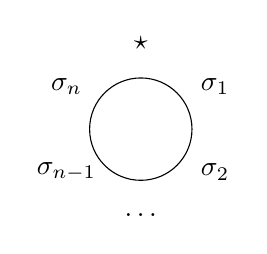
\begin{tikzpicture}
    \draw[black] (0,0) circle(0.65cm);
    \node[draw=none, minimum size=2.5cm, regular polygon, regular
    polygon sides=6] (d) at (0,0) {};
    \draw[fill] (d.side 1) circle (0pt) node{\(\star\)};
    \draw[fill] (d.side 2) circle (0pt) node{\(\sigma_n\)};
    \draw[fill] (d.side 3) circle (0pt) node{\(\sigma_{n-1}\)};
    \draw[fill] (d.side 4) circle (0pt) node{\(\dots\)};
    \draw[fill] (d.side 5) circle (0pt) node{\(\sigma_2\)};
    \draw[fill] (d.side 6) circle (0pt) node{\(\sigma_1\)};
      \end{tikzpicture}
    \]
  \item To each entry \(\sigma_k\), assign an ``index'' \(I_k\)
    recursively as follows \[
      I_k =
      \begin{cases}
        I_{k-1}+1 & \text{ if }\star\text{ is passed going from
        }\sigma_{k-1}\text{ to }\sigma_k\text{ in a clockwise path
          around the circle.} \\
        I_{k-1} & \text{ otherwise.}
      \end{cases}
    \]
  \item Define \(\charge(\sigma) = \sum_{k=1}^n I_k\), that is, the
    sum of the indices.
  \end{enumerate}
\end{defn}
\begin{example}
  The permutation \((6,7,1,4,2,3,5)\) has \[
    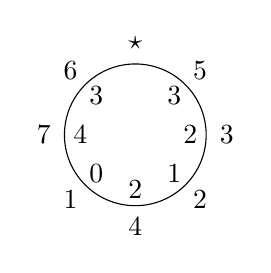
\begin{tikzpicture}
    \draw[black] (0,0) circle(0.9cm);
    \node[draw=none, minimum size=2.5cm, regular polygon, regular
    polygon sides=8] (d) at (0,0) {};
    \draw[fill] (d.side 1) circle (0pt) node{\(\star\)};
    \draw[fill] (d.side 2) circle (0pt) node{\(6\)};
    \draw[fill] (d.side 3) circle (0pt) node{\(7\)};
    \draw[fill] (d.side 4) circle (0pt) node{\(1\)};
    \draw[fill] (d.side 5) circle (0pt) node{\(4\)};
    \draw[fill] (d.side 6) circle (0pt) node{\(2\)};
    \draw[fill] (d.side 7) circle (0pt) node{\(3\)};
    \draw[fill] (d.side 8) circle (0pt) node{\(5\)};

    \node[draw=none, minimum size=1.5cm, regular polygon, regular
    polygon sides=8] (d) at (0,0) {};
    \draw[fill] (d.side 2) circle (0pt) node{\(3\)};
    \draw[fill] (d.side 3) circle (0pt) node{\(4\)};
    \draw[fill] (d.side 4) circle (0pt) node{\(0\)};
    \draw[fill] (d.side 5) circle (0pt) node{\(2\)};
    \draw[fill] (d.side 6) circle (0pt) node{\(1\)};
    \draw[fill] (d.side 7) circle (0pt) node{\(2\)};
    \draw[fill] (d.side 8) circle (0pt) node{\(3\)};
    \end{tikzpicture}
  \]
  charge \(3+4+0+2+1+2+3=15\).
\end{example}
\begin{defn}
  We define the \de{cocharge} of a permutation \(\sigma = (\sigma_1,
  \ldots, \sigma_n)\) to be \[
    \cocharge(\sigma) \defeq \binom{n}{2}-\charge(\sigma)
  \]
  We also define \[
    \comaj(\sigma) = \sum_{i \in \Des(\sigma)}(n-i)
  \]
\end{defn}
\begin{rmk}
  We can also show cocharge can be computed like charge, but with the
  ``opposite'' recurrence 
  relation of charge, which is what we will use to show the
  proposition below.
\end{rmk}
\begin{prop}
  Given a permutation \(\sigma\), \[
    \cocharge(\sigma) = \comaj(\sigma^{-1})
  \]
\end{prop}
\begin{proof}[Idea of Proof]
  Let \(\sigma\) be a permutation with a descent \(k\), that is,
  \(\sigma_k > \sigma_{k+1}\). This adds \(n-k\) to
  \(\comaj(\sigma)\). Then, observe \[
    \sigma = \left(
      \begin{array}{cccccc}
        1&\cdots&k&k+1&\cdots&n\\
        \sigma_1&\cdots&\sigma_k&\sigma_{k+1}&\cdots&\sigma_n
      \end{array}
\right) \to[-1] \sigma^{-1} = \left(
  \begin{array}{cccccc}
    \cdots&\sigma_{k+1}&\cdots&\sigma_k&\cdots\\
    \cdots&k+1&\cdots&k&\cdots
  \end{array}
  \right)
  \]
  That is, \(k+1\) is to the left of \(k\) in \(\sigma^{-1}\). So, our
  cocharge diagram will look like \[
    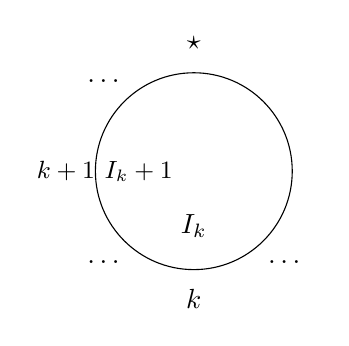
\begin{tikzpicture}
    \draw[black] (0,0) circle(1.25cm);
    \node[draw=none, minimum size=3.5cm, regular polygon, regular
    polygon sides=8] (d) at (0,0) {};
    \draw[fill] (d.side 1) circle (0pt) node{\(\star\)};
    \draw[fill] (d.side 2) circle (0pt) node{\(\dots\)};
    \draw[fill] (d.side 3) circle (0pt) node{\small \(k+1\)};
    \draw[fill] (d.side 4) circle (0pt) node{\(\dots\)};
    \draw[fill] (d.side 5) circle (0pt) node{\(k\)};
    \draw[fill] (d.side 6) circle (0pt) node{\(\dots\)};

    \node[draw=none, minimum size=1.5cm, regular polygon, regular
    polygon sides=8] (d) at (0,0) {};
    \draw[fill] (d.side 3) circle (0pt) node{\small \(I_{k} + 1\)};
    \draw[fill] (d.side 5) circle (0pt) node{\(I_k\)};
    \end{tikzpicture}
  \]
  Therefore, the \(k+1\) occurring before the \(k\) adds \(1\) to
  the index for every number greater than \(k\), which adds \(n-k\) to
  the \(\cocharge(\sigma^{-1})\). 
\end{proof}
\subsection{Dominance Order on Partitions}
\begin{defn}
  Let \(S\) be the set of partitions of degree \(n\), ie whose parts
  sum to \(n\). Then, for \(\lambda,\mu \in S\), the \de{dominance
    order} on \(S\) is given by \[
    \lambda \dominatedby \mu \iff \sum_{i=1}^\ell \lambda_i \leq
    \sum_{i=1}^\ell \mu_i \ \ \forall \ell
  \]
  where \(\lambda = (\lambda_1, \ldots, \lambda_m)\) and \(\mu =
  (\mu_1, \ldots, \mu_k)\).
\end{defn}
\begin{example}
  \((1,1,1,1) \dominatedby (2,2) \dominatedby (4)\) and \((2,2,1)
  \dominates (2,1,1,1)\). Furthermore, \((3,3)\) and \((4,1,1)\) are
  incomparable since \(3 < 4\) but \(3+3=6>5=4+1\).
\end{example}
\begin{defn}
  An partition \(\mu\) \de{covers} \(\lambda\), denoted \(\mu \covers
  \lambda\),  when \(\mu
  \strictlydominates \lambda\) (that is, \(\mu \dominates \lambda, \mu
  \neq \lambda\)) and there is no partition \(\nu\) such that \(\mu
  \strictlydominates \nu \strictlydominates \lambda\).
\end{defn}
\begin{rmk}
  Covering relations are sufficient to define a partial order in
  general. 
\end{rmk}
\begin{prop}
  Given partitions \(\lambda,\mu\) of degree \(n\), \[
    \lambda \dominatedby \mu \iff \lambda' \dominates \mu'
  \]
  where \(\lambda'\) is the conjugate partition to \(\lambda\), and
  similarly for \(\mu'\).
\end{prop}
\begin{proof}
  See \cite{macdonald}*{1.11}.
\end{proof}
\begin{defn}
  The \de{weak order} on \(\Sym_n\) is defined by, for \(\sigma,
  \gamma \in \Sym_n\), \[
    \sigma \coveredby_w \gamma \iff \gamma = \sigma s_i \text{ and
    }\ell(\gamma) = \ell(\sigma)+1
  \]
  where \(s_i\) is the transposition switching \(i\) and \(i+1\).
\end{defn}
\begin{example}
  In one-line notation, \[
    (123) \coveredby (213) = (123)s_1 \coveredby (231) = (213)s_2 = s_1s_2
  \]
  Note that \[
    s_1 = (213) \not\coveredby (312) = s_2s_1
  \]
\end{example}
\begin{defn}
  The \de{strong (Bruhat) order} on \(\Sym_n\) is defined by, for
  \(\sigma, \gamma \in \Sym_n\), \[
    \sigma \coveredby_s \gamma \iff \gamma = \sigma \tau_{ij} \text{ and
    } \ell(\gamma) = \ell(\sigma)+1
  \]
  where \(\tau_{ij}\) is the transposition switching \(i\) and \(j\).
\end{defn}
\begin{thm}[Strong Exchange Property]
  Given \(\sigma \coveredby_s \gamma\) and \(\gamma = s_{i_1} s_{i_2}
  \cdots s_{i_\ell}\), then \(\sigma = s_{i_1} s_{i_2} \cdots
  \hat{s}_{i_k} \cdots s_{i_\ell}\) where the hat means \(s_{i_k}\) is
  deleted from the expression.
\end{thm}
\subsection{Young's Poset on Partitions}
\begin{defn}
  The \de{Young order} on partitions is given by \[
    \lambda \leq \mu \iff \lambda \subset \mu
  \]
  when viewed as Ferrers diagrams. Equivalently, \[
    \lambda \coveredby \mu \iff \mu = \lambda + \text{ an addable corner}
  \]
\end{defn}
\begin{defn}
  Given a rectangle \((m^n)\), the \de{order ideal generated by
    \((m^n)\)} is \(\{\lambda \subset (m^n)\}\) with induced
  containment order.   The \de{rank generating function} is given
  by \[
    \sum_{\lambda \subset (m^n)} q^{|\lambda|}
  \]
  where \(|\lambda| = \sum \lambda_i\).
\end{defn}
\begin{example}
  The induced sub-poset of \((2^3) = (2,2,2)\) is given by \[
    \ytableausetup{boxsize=0.5em}
    \begin{tikzcd}[row sep=tiny, column sep=tiny]
      &&\ydiagram{2,2,2} \ar[d,dash]& \\
      &&\ydiagram{1,2,2} \ar[ld,dash] \ar[rd,dash]&\\
      &\ydiagram{1,1,2} \ar[ld,dash] \ar[rd,dash]&&\ydiagram{2,2} \ar[ld,dash]\\
      \ydiagram{1,1,1}\ar[rd, dash]&&\ydiagram{1,2} \ar[ld,dash]
      \ar[rd,dash]&\\
      &\ydiagram{1,1}\ar[rd,dash]&&\ydiagram{2}\ar[ld,dash]\\
      &&\ydiagram{1}\ar[d,dash]&\\
      &&\emptyset&
    \end{tikzcd}
    \ytableausetup{boxsize=normal}
  \]
  and thus the rank generating function is \[
    1+q+2q^2+2q^3+2q^4+q^5+q^6
  \]
\end{example}
\begin{defn}
  We define the \de{quantum binomial} or \de{Gaussian polynomial} to
  be \[
    \qbinom{m+n}{n} \defeq \frac{[m+n]_q!}{[m]_q![n]_q!}
  \]
\end{defn}
\begin{example}
  \[
    \qbinom{2}{1} = \frac{1+q}{1 \cdot 1} = 1+q
  \]
\end{example}
\begin{prop}
  Given \(m,n \in \N\), we have \[
    \sum_{\lambda \subset (m^n)} q^{|\lambda|} = \qbinom{m+n}{n}
  \]
\end{prop}
\begin{proof}
  The proof is given by an inductive argument on \(m+n\). For the
  inductive step, one breaks up the set \(\{\lambda \subset (m^n)\}\)
  into the set of all \(\lambda\)'s containing a top left cell and the
  set of all \(\lambda\)'s that do not, thus giving \[
    \sum_{\lambda \subset (m^n)} q^{|\lambda|} = \sum_{\lambda \subset
    ((m-1)^n)} q^n q^{|\lambda|} + \sum_{\lambda \subset
    (m^{n-1})} q^{|\lambda|}
  \]
\end{proof}
\section{Tableaux}
\subsection{Tableaux Basics}
\begin{prop}
  A saturated chain in Young's Poset is given by \[
    \emptyset \coveredby \lambda^1 \coveredby \lambda^2 \coveredby
    \cdots \coveredby \lambda^\ell
  \]
  where \(\lambda^i/\lambda^{i-1}\) is one cell.
\end{prop}
\begin{defn}
  A \de{standard Young tableau} of shape \(\lambda\) is given by a
  saturated chain in Young's poset where each
  \(\lambda^i/\lambda^{i-1}\) is filled with the number \(i\).

  Alternatively, one can define a standard Young tableau of shape
  \(\lambda \partitionof n\) to be a filling of \(\lambda\) with
  \(\{1,2,\ldots,n\}\) such that rows and columns are strictly
  increasing.
\end{defn}
\begin{example}
  \[
    \emptyset \coveredby \ydiagram{1} \coveredby \ydiagram{2}
    \coveredby \ydiagram{1,2} \coveredby \ydiagram{1,3} \coveredby
    \ydiagram{2,3} \correspondsto \ytableaushort{35,124}
  \]
\end{example}
\begin{defn}
  Given a partition \(\lambda\), the \de{hook length} of cell \(x =
  (i,j) \in \lambda\), denoted \(h_\lambda(x)\), is given by the
  number of cells in row \(i\) 
  easy of \(x\) plus the number of cells in column \(j\) north of
  \(x\) plus \(1\). 
\end{defn}
\begin{example}
  \[
    \lambda = \ydiagram{1,2,4,4,5,5}*[*(lightgray)]{0,1+1,1+1,2+2}*[*(black)]{0,0,0,1+1}
  \]
  The black shaded cell above has hook length \(2+2+1 = 5\). The
  following diagram is filled in with the hook length of each cell. \[
    \ytableaushort{21,431}
  \]
\end{example}
\begin{prop}
  Let \(f^\lambda\) be the number of standard Young tableaux of shape
  \(\lambda \partitionof n\). Then, \[
    f^\lambda = \frac{n!}{\prod_{x \in \lambda} h_\lambda(x)}
  \]
\end{prop}
\subsection{Robinson-Schensted-Knuth (RSK) Correspondence}
We will discuss a bijection between matrices with entries in \(\N_0\)
with finite support and pairs of semistandard Young tableaux \((\TP,
\TQ)\) of the same shape. 
\begin{defn}
  Let \(\T = (\T_{i,j})\) be a tableau and \(x\) be a positive
  integer. We define 
  \de{row insertion}, denoted \(\T \leftarrow x\) to be the algorithm,
  that takes \(\T\) and adds a cell labeled \(x\) as follows.
  \begin{enumerate}[label=(\arabic*)]
  \item Go to row \(1\). Pick \(r_1\) such that \(\T_{1,r_1-1} \leq x\)
    (if \(\T_{1,1} > x, r_1=1\)).
  \item If \(\T_{1,r_1}\) does not exist, add
    cell labeled \(x\) to the end of the row.
  \item Otherwise, replace \(\T_{1,r_1}\) with \(x\) to get
    \(\T'\). Then, do \(\T' \leftarrow \T_{1,r_1}\) on row \(2\).
  \item Repeat this process until either the bumped entry can be put
    into the end of the row into which it is bumped or until it is
    bumped out of the final row, in which case it will form a new row
    with one entry. 
  \end{enumerate}
\end{defn}
\begin{example}
  Let \[
    \T = \ytableaushort{8,566,1124}
  \]
  Then, \[
    \T \leftarrow 3 = \ytableaushort{8,5,466,1123} \text{ and } \T
    \leftarrow 5 = \ytableaushort{8,566,11245}
  \]
  Explicitly, in the first case, we get the steps \[
    \hspace{-0.5in} \ytableaushort{8,566,1124}*[*(lightgray)]{0,0,3+1}
    \begin{array}{c}
      \\ \\ \\ \\
\leftarrow 3
    \end{array}
,\ 
    \ytableaushort{8,566,1123}*[*(lightgray)]{0,1}
    \begin{array}{c}
      \\ \\
\leftarrow 4 \\ \\
    \end{array}
,\
\ytableaushort{8,466,1123}*[*(lightgray)]{1}
\begin{array}{c}
\leftarrow 5 \\ \\
\end{array}
,\
    \ytableaushort{5,466,1123}
    \begin{array}{c}
\leftarrow 8 \\ \\ \\ \\ \\ 
    \end{array},
    \ytableaushort{8,5,466,1123}
  \]
  Notice that, in both cases, we ended up with a semistandard Young
  tableau. 
\end{example}
\begin{lem}
  If \(\T\) is a semistandard Young tableau, then so is \(\T
  \leftarrow x\). 
\end{lem}
\begin{proof}
  From the algorithm, it is immediate that the rows will still be
  weakly increasing, so we need only check that the columns are
  strictly increasing. To do this, we will define the notion of an
  ``insertion path.''
  \begin{defn}
    The \de{insertion path} or \de{bumping route} of the row-insertion
    \(\T \leftarrow x\) is the 
    collection of the cells \((1,r_1), (2,r_2), \ldots,
    (k,r_k)\) where \((r_1, \ldots, r_k)\) come from the
    row-bumping algorithm.
  \end{defn}
  \begin{example}
    In \[
      \ytableaushort{8,566,1124} \leftarrow 3 = \ytableaushort{8,5,466,1123}
    \]
    the bumping path is \[
      \ytableaushort{8,5,466,1123}*[*(lightgray)]{1,1,1,3+1}
    \]
    or \(((1,4),(2,1),(3,1),(4,1))\).
  \end{example}
  We want to show that the insertion path (starting at row \(1\))
  always moves in a weakly westward direction.

  Let us say an entry \(b\), originally in \(\T_{n,m}\), is bumped into
  \(\T_{n+1,m'}\). If \(m' > m\), then \(m'\) is the largest integer
  such that \(\T_{n+1,m'-1} \leq b\) by the construction of the
  algorithm. So, we have the following picture \[
    \ytableausetup{boxsize=3em}
    \begin{ytableau}
      \scriptstyle \T_{n+1,m} & \cdots & \scriptstyle \T_{n+1,m'}\\
      \scriptstyle \T_{n,m} & \cdots & \T_{n,m'}
    \end{ytableau} \leftrightarrow
    \begin{ytableau}
      >b & \cdots & >b\\
      b & \cdots & \geq b
    \end{ytableau}
    \ytableausetup{boxsize=normal}
  \]
  where we have \(\T_{n,m'} \geq b\) by
  the semistandardness of \(\T\), which also gives \(\T_{n+1,m'} >
  b\). However, this would force \(\T_{n+1,m'-1} > b\), which
  contradicts the inequality \(\T_{n+1,m'-1} \leq b\) above.
\end{proof}
\begin{lem}\label{path-to-the-left}
  Let \(\T\) be a semistandard Young tableau. If \(j \leq k\), then the
  insertion path \(\T \leftarrow j\) is 
  strictly to the left of \((\T \leftarrow j) \leftarrow k\). 
\end{lem}
\begin{rmk}
  This lemma can be strengthened, but we are content with the
  above. See \cite{fulton}*{p 9} for a more complete version. Our
  proof is adapted from the proof in \cite{fulton}.
\end{rmk}
\begin{proof}[Proof of Lemma]
  Suppose \(j \leq k\) and \(j\) bumps an element \(x\) from the first
  row. The element \(y\) bumped by \(k\) from the first row must lie
  strictly to the right of the cell where \(j\) bumped \(x\) by the
  semistandardness of \(\T\) and the construction of the row-bumping
  algorithm. Furthermore, we get \(x \leq y\), and so the argument
  continues from row to row. \[
    \begin{ytableau}
      *(red)& &*(blue) \\
      & &*(red)x&*(blue)y&\\
      & &*(red)j& &*(blue)k& &
    \end{ytableau} 
  \]
\end{proof}
\begin{rmk}
  An important point that underlies the RSK correspondence is that
  this row-bumping process is invertible provided one knows the
  insertion path. For instance, \[
    \ytableaushort{8,5,466,1123}*[*(lightgray)]{1,1,1,3+1}
  \]
  Can be undone by simply shifting every entry in the path down. \[
    \ytableaushort{\none,8,566,1124{\none[3]}}*[*(lightgray)]{1,1,1,3+1}
    \rightarrow \ytableaushort{8,566,1124}, 3
  \]
  In fact, one can do this only knowing the location of the cell that
  has been added to the diagram, simply running the algorithm
  backwards \[
    \ytableaushort{8,5,466,1123}*[*(lightgray)]{1},
    \ytableaushort{5,466,1123}*[*(lightgray)]{1} \leftarrow 8,
    \ytableaushort{8,466,1123}*[*(lightgray)]{0,1} \leftarrow 5,
    \ytableaushort{8,566,1123}*[*(lightgray)]{0,0,3+1} \leftarrow 4,
    \ytableaushort{8,566,1124}, 3 
  \]
  In RSK, we will use another tableau to record this information about
  when boxes were added.
\end{rmk}
\begin{defn}[Robinson-Schensted]
  Given a word \(w = w_1 w_2 \ldots w_\ell\), let \(\TP(w)\) be the
  tableau \[
    \ytableausetup{centertableaux}
    P(w) \defeq ((\ldots((\ytableaushort{{w_1}} \leftarrow w_2)
    \leftarrow w_3) \leftarrow \cdots) \leftarrow w_{\ell-1})
    \leftarrow w_\ell
    \ytableausetup{nocentertableaux}
  \]
  and let \(\TQ(w)\) be the \de{recording tableau} or \de{insertion
    tableau} whose entries are integers \(1, \ldots, \ell\) and where
  \(k\) is placed in the box that is added at the \(k\)th step in the
  construction of \(P(w)\). 
\end{defn}
\begin{example}
  Let \(w = 5482\). Then, we get successive pairs \[
    \ytableaushort{5}\ \ytableaushort{1} \ \ \ \ \ytableaushort{5,4}\
    \ytableaushort{2,1} \ \ \ \ \ytableaushort{5,48}\
    \ytableaushort{2,13} \ \ \ \ \ytableaushort{5,4,28}\
    \ytableaushort{4,2,13}     
  \]
  where the last pair is \((\TP(w), \TQ(w))\).
\end{example}
The fact that this is a correspondence between words and pairs of
tableaux comes from the reversibility of the row-bump combined with
knowing the inserted cell. In the example above, \(\TQ\) is a standard
tableaux. We will prove a more general correspondence, which will get
us what we need about \(\TQ\).
\begin{defn}
  Given a (possibly infinite) matrix \(A\) with entries in \(\N_0\)
  with finite support and nonzero entries , we define \[
    w_A \defeq \left(
      \begin{array}{ccc}
        i_1& \cdots &i_m\\
        j_1& \cdots &j_m
      \end{array}
    \right)
  \]
  in which, for any pair \((i,j)\) that indexes an entry \(A_{i,j}\)
  of \(A\), there are \(A_{i,j}\) columns equal to \(\binom{i}{j}\),
  and all columns satisfy the following two conditions.
  \begin{itemize}
  \item \(i_1 \leq \cdots \leq i_m\) and
  \item If \(i_r = i_s\) and \(r \leq s\), then \(j_r \leq j_s\).
  \end{itemize}
\end{defn}
\begin{example}
  \[
    A = \left(
      \begin{array}{ccc}
        1&0&2\\
        0&3&1\\
        0&0&1
      \end{array}
    \right) \rightarrow w_A = \left(
      \begin{array}{cccccccc}
        1&1&1&2&2&2&2&3\\
        1&3&3&2&2&2&3&3
      \end{array}
    \right)
  \]
\end{example}
\begin{defn}[Robinson-Schensted-Knuth]
  Given a matrix \(A\) with entries in \(\N_0\) with finite support,
  construct \[
    w_A = \left(
      \begin{array}{ccc}
        i_1&\ldots&i_m\\
        j_1&\ldots&j_m
      \end{array}
    \right)
  \]
  Then, we will construct a sequence of pairs of tableau were \[
    (\TP^0, \TQ^0) = (\emptyset, \emptyset), \TP^{t+1} = \TP
    \leftarrow j_{t+1}, 
  \]
  and \(\TQ^{t+1} = \TQ^t\) with \(i_{t+1}\) added
  in the cell that appeared by doing the insertion for
  \(\TP^{t+1}\). Then, we say that \(A\) corresponds to \((\TP^m, \TQ^m)\).
\end{defn}
\begin{example}
  Continue with \(A,w_A\) as in the example above. Then,
  \begin{align*}
    (\TP^0, \TQ^0)
    & = \left( \emptyset, \emptyset \right) \\
    (\TP^1, \TQ^1)
    & = \left( \ytableaushort{1}, \ytableaushort{1} \right) \\
    (\TP^2, \TQ^2)
    & = \left( \ytableaushort{13},
      \ytableaushort{11}*[*(lightgray)]{1+1} \right) \\
    (\TP^3, \TQ^3)
    & = \left( \ytableaushort{133},
      \ytableaushort{111}*[*(lightgray)]{2+1} \right)\\
    (\TP^4, \TQ^4)
    & = \left( \ytableaushort{3,123}, \ytableaushort{2,111} \right)\\
    (\TP^5, \TQ^5)
    & = \left( \ytableaushort{33,122}, \ytableaushort{22,111} \right)\\
    (\TP^6, \TQ^6)
    & = \left( \ytableaushort{33,1222}, \ytableaushort{22,1112}
      \right) \\
    (\TP^7, \TQ^7)
    & = \left( \ytableaushort{33,12223}, \ytableaushort{22,11122}
      \right)\\
    (\TP^8, \TQ^8)
    & = \left( \ytableaushort{33,122233}, \ytableaushort{22,111223} \right)
  \end{align*}
\end{example}
\begin{lem}
  \(\TQ^t\) constructed above is a semistandard Young tableau.
\end{lem}
\begin{proof}
  The rows of \(\TQ^t\) are certainly weakly increasing since the
  first row of \(w_A\) is weakly increasing by construction. For
  columns strictly increasing, we observe that if \(i_k = i_{k+1}\),
  then \(j_k \leq j_{k+1}\), and so by lemma \ref{path-to-the-left},
  we get that the insertion path \(M \leftarrow j_k\) is strictly to
  the left of \((M \leftarrow j_k) \leftarrow j_{k+1}\) and so the
  columns must be strictly increasing.
\end{proof}
\begin{thm}
  The RSK correspondence is a actual correspondence between matrices
  with entries in \(\N_0\) with finite support and pairs of
  semistandard Young tableaux of the same shape.
\end{thm}
\begin{proof}
  To show we have a correspondence, we will construct an inverse
  algorithm. Given \((\TP, \TQ) = (\TP^m, \TQ^m)\), we do the
  following.
  \begin{enumerate}[label=(\arabic*)]
  \item Consider \(\TQ_{r,s}\), the rightmost entry of the largest
    element in \(\TQ\) (since \(\TQ\) can have repeated entries). Then,
    set \(\TQ^{m-1} = \TQ^m \setminus \TQ_{r,s}\).
  \item \(\TP_{r,s}\) is the last spot in the insertion path of
    \(\TP^{m-1} \leftarrow j_m\).
  \item We need \(\TP_{r-1,t}\), the rightmost element of row \(r-1\)
    that is smaller than \(\TP_{r,s}\). Then, do reverse bumping until
    you get \(j_m\).
  \item Repeat this process until \(w_A\) is recovered.
  \end{enumerate}
  \begin{example}
    \begin{enumerate}
    \item     \[
      \TQ = \ytableaushort{22,111}*[*(lightgray)]{1+1} \implies i_5 = 2
    \]
    \item \[
      \TP = \ytableaushort{33,122}*[*(lightgray)]{1+1}
    \]
  \item \[
      \ytableaushort{3,122}*[*(lightgray)]{0,2+1} \leftarrow 3,
      \ytableaushort{3,123} \text{ and } j_5 = 2
    \]
    \end{enumerate}
  \end{example}
  We also want to show that this inverse is well-defined, that is, if
  \(i_k = i_{k+1}\), then \(j_k \leq j_{k+1}\). If \(i_k = \TQ_{r,s}\)
  and \(i_{k+1} = \TQ_{u,v}\), then \(r \geq u\) and \(s < v\). Then,
  it must be that the inverse insertion path of \(\TP_{r,s}\) is
  strictly to the left of the insertion path of \(\TP_{u,v}\). Thus,
  we get, in the first row, \[
\ytableaushort{{j_k}\cdots{\scriptstyle j_{k+1}}} \implies j_k \leq j_{k+1}
  \]
\end{proof}
\section{Symmetric Polynomials and Symmetric Functions}
\subsection{Introduction to Symmetric Polynomials}
Let \(R\) be a commutative ring with unity and let \(x_1, x_2, \ldots,
x_n\) be indeterminates.
\begin{defn}
  The ring of polynomials in \(n\) variables with coefficients in
  \(R\) is \[
    R[x_1, x_2, \ldots, x_n] = \left\{ \sum c_\alpha x^\alpha \st
      \alpha \in \N^n \right\} \text{ where } x^\alpha =
    x_1^{\alpha_1} x_2^{\alpha_2} \cdots x_n^{\alpha_n}
  \]
  with multiplication \(x^\alpha x^\beta = x^{\alpha+\beta}\).
\end{defn}
\begin{defn}
  We say \(f \in R[x_1, \ldots, x_n]\) has \de{homogeneous degree \(d\)}
  if \[
    f = \sum_{|\alpha|=d} c_\alpha x^\alpha
  \]
\end{defn}
\begin{example}
  \(3x_1^2+19x_1x_3\) has degree \(2\).
\end{example}
\begin{prop}
  Let \[
    R^d[x_1, \ldots, x_n] := \{f \in R[x_1, \ldots, x_n]\ \st f \text{
      has degree }d\}
\]
Then, \(R[x_1, \ldots, x_n]\) is a graded ring with \[
  R[x_1, \ldots, x_n] = \bigoplus_{d \geq 0} R^d[x_1, \ldots, x_n]
\]
\end{prop}
\begin{proof}
  Let \(f \in R^a[x_1, \ldots, x_n]\) and \(g \in R^b[x_1, \ldots,
  x_n]\). Then, \(fg \in R^{a+b}[x_1, \ldots, x_n]\).
\end{proof}
\begin{prop}
  There is a degree preserving \(\Sym_n\)-action on \(R[x_1, \ldots,
  x_n]\) given by \[
    \sigma.f(x_1, \ldots, x_n) = f(x_{\sigma(1)}, \ldots, x_{\sigma(n)})
  \]
  for \(\sigma \in \Sym_n\). 
\end{prop}
\begin{example}
  Let \(\sigma = (1,3,2)\) in one-line notation. Then, for \[
    g(x) = 3x_1^2+19x_1x_3-7x_1+18x_2x_3^4 \in \Z[x_1,x_2,x_3]
  \]
  we have \[
    \sigma g = 3x_1^2+19x_1x_2-7x_1+18x_2^4x_3
  \]
\end{example}
\begin{defn}
  The \de{ring of symmetric polynomials} on \(n\) indeterminates is \[
    \sym_n := \{f \in R[x_1, \ldots, x_n]\ \st \sigma f = f\ \forall
  \sigma \in \Sym_n\} 
  \]
  This is a subring of \(R[x_1, \ldots, x_n]\) and is sometimes
  denoted \(R[x_1, \ldots, x_n]^{\Sym_n}\) (meaning \(\Sym_n\)-action
  fixed points).
\end{defn}
\begin{example}
  \(x_1+x_2+x-3\) and \(3x_1^2+3x_2^2+3x_3^2-9x_1x_2x_3\) are both in
  \(\sym_3\). However, \(x_1+x_2\) is not in \(\sym_3\) since the
  permutation \((1,3,2)\) (one-line) yields \(x_1+x_3\).
\end{example}
\begin{cor}
  \[
    \sym_n = \bigoplus_{d \geq 0} \sym_n^d \text{ where } \sym_n^d :=
    \{f \in \sym_n \st f \text{ has degree }d\}
  \]
  Furthermore, if \(R\) is a field, say \(\k\), then \(\sym_n\) is a
  graded algebra since \(\k[x_1, \ldots, x_n]\) is a graded algebra.
\end{cor}
\begin{rmk}
  In particular, this makes \(\sym_n\) a vector space over
  \(\k\). Thus, we can ask about various \(\k\)-bases of \(\sym_n\).
\end{rmk}
\begin{defn}
  For \(\lambda \partitionof d\), the monomial symmetric polynomial
  is \[
    m_\lambda(x_1, \ldots, x_n) \defeq \sum_{\substack{\alpha \in \N^n
      \\ \alpha \sim \lambda}} x^\alpha
  \]
\end{defn}
\begin{example}
  \begin{itemize}
  \item   \(m_1(x_1, x_2) = x_1+x_2\) since \((1,0) \sim (0,1)\).
  \item \(m_{211}(x_1, x_2, x_3) = x_1^2 x_2 x_3 + x_1 x_2^2 x_3 + x_!
    x_2 x_3^2\) since \((211) \sim (121) \sim (112)\).
  \item \(m_{211}(x_1, x_2) = 0\) because there is no partition with
    \(2\) parts that can be rearranged to \((2,1,1)\).
  \end{itemize}
\end{example}
\begin{prop}
  \(\{m_\lambda(x_1, \ldots, x_n)\}_{\lambda \partitionof d}\) is a
  basis for \(\sym_n^d\).
\end{prop}
\begin{proof}
  Each element of our set is symmetric since every monomial
  coefficient is \(1\) and every permutation of \(x^\lambda\) occurs
  in \(m_\lambda\). Also, linear independence is immediate; each
  \(m_\lambda\) has unique monomials. Thus, it suffices to show that
  monomial symmetric polynomials span \(\sym_n^d\). \\

  Given \(f \in \sym_n^d\), we write \[
    f = \sum_{|\alpha|=d} c_\alpha x^\alpha \text{ where } c_\alpha =
    c_{\sigma(\alpha)}, \forall \sigma \in \Sym_n
  \]
  In particular, \(c_\alpha = c_\lambda\) for \(\alpha \sim
  \lambda\). In otherwords, \(\lambda\) is a partition rearrangement
  of \(\alpha\) Thus, \[
    f = \sum_{\lambda \partitionof d} c_\lambda \left( \sum_{\alpha
        \sim \lambda} x^\alpha \right) = \sum_{\lambda \partitionof d}
    c_\lambda m_\lambda(x_1, \ldots, x_n)
  \]
\end{proof}
\begin{cor}
  An immediate corollary to this result is that any basis for
  \(\sym_n^d\) can be indexed by \(\lambda \partitionof d\).
\end{cor}
\begin{defn}
  For \(\alpha\) a partition, we establish the convention \[
    x^\alpha \defeq x_1^{\alpha_1} x_2^{\alpha_2} \cdots x_n^{\alpha_n}
  \]
\end{defn}
\begin{defn}
  For \(r \geq 0\), \de{elementary symmetric polynomial} \[
    e_r(x_1, x_2, \ldots, x_n) \defeq \sum_{1 \leq i_1 < i_2 < \cdots < i_r
    \leq n} x_{i_1} x_{i_2} \cdots x_{i_r}
  \]
  and, for \(\lambda \partitionof d\) with \(\lambda = (\lambda_1,
  \ldots, \lambda_\ell)\), \[
    e_\lambda(x_1, \ldots, x_n) = e_{\lambda_1}(x_1, \ldots, x_n)
    e_{\lambda_2}(x_1, \ldots, x_n) \cdots e_{\lambda_\ell}(x_1,
    \ldots, x_n)
  \]
\end{defn}
\begin{example}
  \begin{align*}
    e_1(x_1, x_2, x_3) = & x_1+x_2+x_3 = m_1(x_1, x_2, x_3)\\
    e_2(x_1, x_2, x_3) = & x_1x_2+x_1x_3+x_2x_3 = m_{11}(x_1, x_2,
                         x_3)\\
    e_{21}(x_1,x_2,x_3) = & (x_1x_2+x_1x_3+x_2x_3)(x_1+x_2+x_3)\\
                       = & x_1^2x_2+x_1x_2^2+x_1x_2x_3+\\
                       & x_1^2x_3+x_1x_2x_3+x_1x_3^2+\\
                       & x_1x_2x_3+x_2^2x_3+x_2x_3^2\\
    = & m_{21}(x_1,x_2,x_3) + 3m_{111}(x_1,x_2,x_3)
  \end{align*}
\end{example}
\begin{prop}
  \(e_r = m_{1^r}\) and \(\{e_r(x_1, \ldots, x_n)\}_{r \in \N}\)
  cannot form a basis of \(\sym\).
\end{prop}
\begin{proof}
  By definition, the elementary symmetric polynomials \(e_r\) are
  symmetric polynomials with degree \(r\) monomials with no variable
  occurring more than once in each monomial. Thus, it must be that
  \(e_r = m_{1^r}\). Furthermore, by the corollary to the monomial
  symmetric polynomials forming a basis, it must be that \(\{e_r\}_{r
    \in \N}\) cannot form a basis because each \(e_r \in \sym_n^r\)
  and so there simply are not enough in each \(\sym_n^d\) to form a basis.
\end{proof}
\begin{prop}
  The set \(\{e_\lambda(x_1, \ldots, x_n)\}_{\lambda \partitionof d}\)
  is a basis for \(\sym_n^d\).
\end{prop}
\begin{proof}
  Since this set is indexed by \(\lambda \partitionof d\), it suffices
  to show that the set spans \(\sym_n^d\). Since \(\{m_\lambda\}\) is
  a basis, it suffices to show \[
    m_\lambda = \sum c_{\lambda,\mu} e_\mu
  \]
  for some \(c_{\lambda,\mu}\). Instead, we will show that \[
    e_\eta = \sum M_{\eta,\mu} m_\mu \text{ and }
    (M_{\eta,\mu})_{\eta,\mu} \text{ is a unitriangular matrix}
  \]
  To do this, we will need the combinatorics of \((0,1)\)-matrices.
  \begin{defn}
    Given a matrix \((0,1)\)-matrix \(A\), let the \de{row sum} be \[
      \row(A) \defeq (r_1, f_2, \ldots, r_n), r_i = \text{number of
        1's in row }i 
    \]
    and \de{column sum} be \[
      \col(A) \defeq (c_1, \ldots, c_n), c_j = \text{number of 1's in
        row }j
    \]
    Finally, let \(B_{\alpha \beta}\) be the number of \((0,1)\)
    matrices with row sum vector \(\alpha\) and column sum vector
    \(\beta\). 
  \end{defn}
  \begin{example}
    Some matrices with \(\row(A) = (2,1,1,0)\) \[
      \left(
        \begin{array}{cccc}
          1&1&0&0\\
          1&0&0&0\\
          1&0&0&0\\
          0&0&0&0
        \end{array}
      \right),
            \left(
        \begin{array}{cccc}
          1&1&0&0\\
          0&1&0&0\\
          1&0&0&0\\
          0&0&0&0
        \end{array}
      \right),
      \left(
        \begin{array}{cccc}
          1&1&0&0\\
          1&0&0&0\\
          0&0&1&0\\
          0&0&0&0
        \end{array}
      \right),
            \left(
        \begin{array}{cccc}
          1&1&0&0\\
          1&0&0&0\\
          0&1&0&0\\
          0&0&0&0
        \end{array}
      \right)
    \]
    The second and fourth matrices have \(\col(A) = (2,2,0,0)\).
  \end{example}
  Then, we claim \[
    e_{\nu'} = m_\nu + \sum_{\nu \strictlydominates \mu} B_{\nu' \mu} m_\mu
  \]
  To do this, first consider one term. Let \(A^*\) be the
  \((0,1)\)-matrix with row sum \(\nu'\) where all the one's are left
  justified.
  \begin{example}
    If \(\nu' = (2,1,1,0)\), then \[
      A^* = \left(
        \begin{array}{cccc}
          1&1&0&0\\
          1&0&0&0\\
          1&0&0&0\\
          0&0&0&0
        \end{array}
      \right)
    \]
    Note that \(\col(A^*) = (3,1) = \nu\)
  \end{example}
  Such an element has \(\col(A^*) = \nu\) and it is the unique
  \((0,1)\)-matrix with \(\row(A) = \nu'\) and \(\col(A) = \nu\). In
  particular, if \(A\) has \(\nu_1\) ones in column one and \(\row(A)
  = \nu;\), the first \(\ell(\nu')=\nu_1\) rows have ones. Thus, all
  ones in column \(1\) are north justified. Iterating this process
  gives the uniqueness result. Any other matrix \(A\) with
  \(\row(A)=\nu'\) will have column sum smaller in dominance than
  \(\nu'\) since the ones in \(A^*\) are pushed all the way to the left.

  Thus, let \(\eta = \nu'\). Then,
  \begin{align*}
    e_\eta
    & = e_{\eta_1}(x_1, \ldots, x_n) e_{\eta_2}(x_1, \ldots, x_n)
      \cdots e_{\eta_\ell}(x_1, \ldots, x_n) \\
    & = \left( \sum_{i_1 < i_2 < \cdots < i_{\eta_1}} x_{i_1} \cdots
      x_{i_{\eta_1}}\right) \left( \sum_{j_1 < j_2 < \cdots < j_{\eta_2}}
      x_{j_1} \cdots x_{j_{\eta_2}}\right) \cdots \left( \sum_{z_1 <
      \cdots < z_{\eta_\ell}} x_{z_1} \cdots x_{z_{\eta_\ell}} \right)
    \\
    & = \sum_{\substack{\alpha\text{ obtained by choosing} \\ i_1 <
    i_2 < \cdots < i_{\eta_1}\\
    j_1 < j_2 < \cdots < j_{\eta_2}  \\
    \vdots \\ z_1 < z_2 < \cdots < z_{\eta_\ell}}} x^{\col(X)}
    \text{ where } X = \left(
    \begin{array}{cccc}
      x_1&\mathcircled{x_2}&\cdots&\mathcircled{x_n}\\
      \mathcircled{x_1}&\mathcircled{x_2}&\cdots&x_n\\
      \vdots&\vdots&&\vdots\\
      {x_1}&\mathcircled{x_2}&\cdots&x_n
    \end{array}
   \right) =
   \left(
\begin{array}{cccc}
  0&1&\cdots&1\\
  1&1&\cdots&0\\
  \vdots&\vdots&&\vdots\\
  0&1&\cdots&0
\end{array}
\right)
  \end{align*}
  where the circled entries are the \(i_1, i_2, \ldots, i_{\eta_1}\)
  entries of row \(1\), the \(j_1, j_2, \ldots, j_{\eta_2}\) entries
  of row \(2\), etc. and thus \[
    e_\eta = \sum_{\substack{A \in \{(0,1)\text{-matrices with
      }\\\row(A)=\eta\}}} x^{\col(A)} = \sum_{\mu \partitionof d}
    \sum_{\substack{(0,1)\text{-matrices } A \\ \text{ with
        }\row(A)=\eta,\\ 
      \col(A)=\mu}} m_{\mu} = \sum_{\mu \partitionof d} B_{\eta, \mu} m_{\mu} 
  \]
  \begin{example}
    \[
      e_{211} = (x_1 x_2 + x_1 x_3 + x_2
      x_3)(x_1+x_2+x_3)(x_1+x_2+x_3) = \sum_{\alpha = \col(A)} x^\alpha 
    \]
    So for instance, \[
      \begin{tikzcd}[ampersand replacement=\&]
   \left(
        \begin{array}{ccc}
          x_1&\mathcircled{x_2}&\mathcircled{x_3}\\
          \mathcircled{x_1}&x_2&x_3\\
          \mathcircled{x_1}&x_2&x_3
        \end{array}
      \right) \ar[r] \ar[d, leftrightarrow] \& x^{\col(A)} = x_1^2x_2x_3 \\
      \left(
        \begin{array}{ccc}
          0&1&1\\
          1&0&0\\
          1&0&0
        \end{array}
\right)
      \end{tikzcd}
    \]
  \end{example}
\end{proof}
\begin{cor}[Fundamental Theorem of Symmetric Polynomials]
  \(\sym_n\) with coefficients in \(R\) is a polynomial ring in the
  \(n\) elementary symmetric polynomials, that is, \(\sym_n \isom
  R[e_1, \ldots, e_n]\) as commutative rings.
\end{cor}
\begin{proof}
  By the above, for \(f \in \sym_n^d\), we write \[
    f = \sum_{\mu \partitionof d} c_\mu e_\mu(x_1, \ldots, x_n)
  \]
  However, since \(e_{\mu_1}, e_{\mu_2}, \ldots, e_{\mu_n}\) commute,
  define \(e^\alpha \defeq e_1^{\alpha_1} e_2^{\alpha_2} \cdots
  e_n^{\alpha_n}\).
  \begin{example}
    \(e_{3222} = e_3e_2e_2e_2 = e_1^0 e_2^3 e_3^1 = e^{(031)}\).
  \end{example}
  Then, we get that \[
    f = \sum c_\mu e^\alpha
  \]
  where \(\alpha_1\) is the number of \(1\)'s in \(\mu\), \(\alpha_2\)
  is the number of \(2\)'s in \(\mu\), etc. This shows that \(f \in
  R[e_1, \ldots, e_n]\). Thus, \(\sym_n^d \subset R[e_1, \ldots,
  e_n]\). However, since \(e_1, \ldots, e_n\) are all symmetric, it
  must be that \(R[e_1, \ldots, e_n] \subset \sym_n\). Thus, we get
  the desired isomorphism.
\end{proof}
\begin{defn}
  For \(r \in \N\), the \de{complete symmetric polynomial} is \[
    h_r(x_1, \ldots, x_n) \defeq \sum_{1 \leq i_1 \leq \cdots \leq i_r
    \leq n} x_{i_1} \cdots x_{i_r}
  \]
  and, for \(\lambda\) a partition, the \de{homogeneous symmetric
    polynomials} are \[
    h_\lambda \defeq h_{\lambda_1} h_{\lambda_2} \cdots h_{\lambda_\ell}
  \]
\end{defn}
\begin{example}
  \begin{align*}
    h_1(x_1,x_2,x_3) & = x_1 + x_2 + x_3 \\
    h_2(x_1,x_2,x_3) & = x_1^2 + x_1x_2 + x_2^2 + x_2x_3 + x_3^2 +
                       x_1x_3\\
    & = m_2(x_1,x_2,x_3) + m_{11}(x_1,x_2,x_3)
  \end{align*}
\end{example}
\begin{prop}
  \(h_r(x_1, \ldots, x_n) = \sum_{\lambda \partitionof r} m_\lambda\)
\end{prop}
\begin{proof}
  This follows immediately by grouping the terms of \(h_r\)
  appropriately. 
\end{proof}
We now wish to show the following.
\begin{prop}\label{homogeneous-are-basis}
  \(\{h_\lambda(x_1,\ldots,x_n)\}_{\lambda \partitionof d}\) is a
  basis for \(\sym_n^d\).
\end{prop}
We will give a proof by generating functions. 
\begin{lem}
  We have the following generating functions
  \begin{align*}
    E(t) & = \prod_i (1+x_i t) = \sum_{k \geq 0} t^k e_k \\
    H(t) & = \frac{1}{\prod_i (1-x_i t)} = \sum_{k \geq 0} t^k h_k
  \end{align*}
\end{lem}
\begin{proof}[Proof of Lemma]
  Observe first
  \begin{align*}
    E(t) & = \prod_i (1+x_i t) \\
         & = (1+x_1 t)(1+x_2 t) \cdots (1+x_n t) \\
    & = \sum_{1 \leq i_1 < \cdots < i_k \leq n} t^j x_{i_1} x_{i_2}
      \cdots x_{i_k} \\
    & = \sum_{k \geq 0} t^k e_k
  \end{align*}
  For \(H(t)\), recall the geometric series identity \[
    \frac{1}{1-x_i t} = \sum_{k \geq 0} x_i^k t^k
  \]
  and thus \[
    \prod \frac{1}{1-x_i t} = \prod_i \left( \sum_{k \geq 0} x_i^k t^k
    \right) = \sum_{k \geq 0} t^k h_k
  \]
\end{proof}
\begin{proof}[Proof of Proposition \ref{homogeneous-are-basis}]
  Since \(H(t) = \frac{1}{E(-t)}\), we get
  \begin{align*}
    H(t)E(-t) = 1
    & \implies \left(\sum_i t^i h_i\right)\left( \sum_j (-t)^j e_j
      \right) = 1 + \sum_{k \geq 1} 0 \cdot t^k \\
    & \implies \sum_{j = 0}^n (-1)^j h_{n-j} e_j = 0, \forall n > 0
  \end{align*}
  So, we check
  \begin{align*}
    n=1\colon & h_1-e_1 = 0 \implies e_1 = h_1 \\
    n=2\colon & h_2-e_1 h_1 + e_2 = 0 \implies e_2 = e_1 h_1 - h_2 = h_1^2-h_2
  \end{align*}
  and so we can iterate to show that \(e_r\) is a sum of
  \(h_\mu\)'s. Thus, we get that \(\{h_\mu\}\) spans \(\sym_n\).
\end{proof}
\subsection{Symmetric Functions}
Notice that we can always get a homomorphism of rings \[
  \sym_{n+1} \onto \sym_n
\]
by setting \(x_{n+1} = 0\). 
\begin{example}
  \begin{align*}
    e_{21}(x_1, x_2, x_3, x_4)
    & = (x_1 x_2 + x_1 x_3 + x_1 x_4 + \cdots)(x_1+x_2+x_3+x_4) \\
    & = m_{21}(x_1, x_2, x_3, x_4) + 3 m_{111}(x_1, x_2, x_3, x_4) \\
    \mapsto e_{21}(x_1, x_2, x_3)
    & = (x_1 x_2 + x_1 x_3 + x_2 x_3)(x_1+x_2+x_3)\\
    & = m_{21}(x_1, x_2, x_3) + 3 m_{111}(x_1, x_2, x_3)
  \end{align*}
\end{example}
In fact, one can check that \(m_\lambda(x_1, \ldots, x_{n+1}) \mapsto
m_{\lambda}(x_1, \ldots, x_n)\) which is nontrivial provided
\(\ell(\lambda) > n\). Thus,
\begin{prop}
  \(\sym_n^d \isom \sym_{n+1}^d\) as \(R\)-modules provided \(n \geq d\).
\end{prop}
Thus, the number of variables we work in is largely irrelevant
provided there are sufficiently many. In order to avoid this formal
annoyance, we will often work with ``infinite symmetric polynomials'',
which we will construct in this following section.
\begin{defn}
  Let \(R\) be a commutative ring with unity. Then, for an infinite
  collection of indeterminates
  \(\{x_1, x_2, \ldots\}\), we say
  \(R[[x_1,x_2,\ldots]]\) is the \de{ring of formal series over \(R\)}
  with elements given as (formal) infinite sums of monomials in the
  indeterminates, addition given by componentwise addition, and
  multiplication given by extension of polynomial multiplication.
\end{defn}
Note that multiplication is well-defined since, given a product of
infinite series \[
\left( \sum_{\alpha \in \N^\infty} c_\alpha x^\alpha
\right)\left( \sum_{\beta \in \N^\infty}
  d_\beta x^\beta \right),
\] the coefficient at \(x^\gamma\)  for \(\gamma \in \N^\infty\) has only
finitely many contributions from the \(c_\alpha\) and \(d_\beta\)'s.
\begin{defn}
  Given \(\alpha, \beta \in \N^\infty\), we say \(\alpha \sim \beta\)
  if the underlying multisets of entries are equal (not counting \(0\)).
\end{defn}
\begin{example}
  \((2,0,1,0) \sim (1,2,0)\)
\end{example}
\begin{defn}
  We say \(f \in R[[x_1, x_2, \ldots]]\)  is a \de{symmetric infinite
    series} if the coefficient of \(x^\alpha\) is equal to the
  coefficient of \(x^\beta\) when \(\alpha \sim \beta\).
\end{defn}
\begin{example}
  The element \(\displaystyle \sum_{d \geq 0} \sum_{i \geq 1} x_i^d\) is a symmetric
  infinite series.
\end{example}
\begin{defn}
  A \de{symmetric polynomial in infinitely many variables} (usually called
  a \de{symmetric function}) is a symmetric infinite series with bounded
  degree. The set of these symmetric polynomials forms a ring of
  symmetric functions, denoted \(\Lambda\).
\end{defn}
\begin{example}
  Let \(b \in \N\). Then, \(\displaystyle \sum_{d \geq 0}^b \sum_{i \geq 1} x_i^d\)
  is a symmetric function.
\end{example}
\begin{rmk}
  For the categorically inclined, the symmetric functions can also be
  constructed as an inverse limit 
  by taking \[
    \sym^d = \lim_{\substack{\leftarrow \\ n}} \sym_n^d
  \]
  in the category of \(\Z\)-modules and then setting \[
    \sym = \bigoplus_{k \geq 0} \sym^k
  \]
  This requires setting up the necessary maps, but this is not so hard
  given the above for those who wish to use inverse limits. Note,
  however, that \(\sym\) is \emph{not} the inverse limit of 
  \(\sym_n\) in the category of rings; such an inverse limit would be
  the ring of symmetric infinite series. However, \(\sym\) would be
  the inverse limit of \(\sym_n\) in the category of graded rings.
\end{rmk}
We wish to extend our definitions for bases of symmetric polynomials
to our ring of symmetric functions.
\begin{defn}
  Let \(\ov{x} = (x_1, x_2, \ldots)\). Then, we define
  \begin{enumerate}
  \item for \(\lambda\) a partition, \[
      m_\lambda(\ov{x}) = \sum_{\alpha \sim \lambda} x^\alpha
    \]
  \item for \(r \in \N\), \[
      e_r(\ov{x}) = \sum_{1 \leq i_1 < i_2 < \cdots < i_r}
      x_{i_1} x_{i_2} \cdots x_{i_r}
    \]
  \item for \(r \in \N\), \[
      h_r(\ov{x}) = \sum_{|\lambda|=r} m_\lambda = \sum_{1 \leq i_1
        \leq i_2 \leq \cdots \leq i_r} x_{i_1} x_{i_2} \cdots x_{i_r}
    \]
  \end{enumerate}
\end{defn}
\begin{example}
  \(h_2(\ov{x}) = m_{(2)}(x) + m_{(1,1)}(x) = x_1^2 + x_2^2 + \cdots + x_1 x_2 + x_1 x_3 + \cdots
  + x_2 x_3 + \cdots\)
\end{example}
Finally, we wish to introduce one more family of symmetric functions.
\begin{defn}
  For any \(r \in \N\), we define the \de{power symmetric
    functions} \[
    p_r \defeq \sum_i x_i^r
  \]
  and, for any partition \(\lambda\), we define \[
    p_\lambda = \prod_i p_{\lambda_i}
  \]
\end{defn}
\begin{prop}
  The generating function for the \(p_r\) is \[
    P(t) = \sum \frac{x_i}{1-x_i t}
  \]
  and also satisfies the identities \[
    P(t) = \frac{H'(t)}{H(t)} \ \ P(-t) = \frac{E'(t)}{E(t)}
  \]
\end{prop}
\begin{proof}
  By direct computation, we see \[
    P(t) \defeq \sum_{r \geq 1} p_r t^{r-1} = \sum_{i \geq 1} \sum_{r
      \geq 1} x_i^r t^{r-1} = \sum_{i \geq 1} \frac{x_i}{1-x_i t}
  \]
  Furthermore, if we are clever at manipulating generating functions,
  we see \[
    P(t) = \sum_{i \geq 1} \frac{d}{dt} \log\left( \frac{1}{1-x_i t}
    \right) = \frac{d}{dt} \log\left( \prod_{i \geq 1} \frac{1}{1-x_i
        t}\right) = \frac{d}{dt} \log(H(t)) = \frac{H'(t)}{H(t)}
  \]
  and \[
    P(-t) = \sum_{i \geq 1} \frac{d}{dt} \log(1+x_i t) =
    \frac{d}{dt}\log\left( \prod_{i \geq 1}(1+x_i t) \right) =
    \frac{d}{dt}\log E(t) = \frac{E'(t)}{E(t)}
  \]
\end{proof}
\begin{cor}[Newton's Identities]
  We have the following identities \[
    nh_n = \sum_{r=1}^n p_r h_{n-r}, \ \ \ n e_n = \sum_{r=1}^n
    (-1)^{r-1}p_r e_{n-r}
  \]
\end{cor}
\begin{proof}
  These come from the proposition above by rearranging and
  expanding. For instance, \[
    H'(t) = P(t)H(t) \implies \sum_{i \geq 1} ih_i t^{i-1} = \left(
      \sum_{r \geq 1} p_r t^{r-1} \right)\left( \sum_{j \geq 1} h_j t^j \right)
  \]
  and so, fixing a specific \(n\), we have \[
    nh_n = \sum_{r+j=n} p_r h_j
  \]
  giving us the desired identity.
\end{proof}
\begin{thm}
  The set \(\{p_\lambda\}_{\text{all partitions }\lambda}\) is a basis
  for \(\sym\) over a field of characteristic \(0\).
\end{thm}
\begin{proof}
  By Newton's identities, \[
    p_n = \sum_{j=1}^n e_j p_{n-j}
  \]
  if we rewrite this recurrence, we get \[
    e_n = \frac{1}{n}\sum_{j=1}^n (-1)^{j-1} e_{n-j} p_j
  \]
  Thus, each \(e_n\) can be written as a rational linear combination
  of the power sums, giving that \(\sym_n \subset \Q[p_1, \ldots,
  p_n]\). Therefore, the \(p_\lambda\)'s form a basis and because
  every power sum polynomial is symmetric, \(\sym_n \isom \Q[p_1,
  \ldots, p_n]\).
\end{proof}
\begin{rmk}
  An alternative proof is just to let \(C=(c_{\lambda,\mu})\) be a
  matrix expressing \(p_\lambda\) in terms of the monomial basis. One
  argues that \[
    p_{\lambda} = c_{\lambda \lambda}m_{\lambda} + \sum_{\mu
      \strictlydominates \lambda} c_{\lambda \mu} m_{\mu}
  \]
  with \(c_{\lambda \lambda} \neq 0\). Then, if \(x_1^{\mu_1} \cdots
  x_m^{\mu_m}\) appears in \[
    p_\lambda = (x_1^{\lambda_1} + x_2^{\lambda_2} +
    \cdots)(x_1^{\lambda_2}+x_2^{\lambda_2}+ \cdots )+\cdots
  \]
  then each \(\mu_i\) must be a sum of \(\lambda_j\)'s, thus making
  \(\mu\) larger in dominance order than \(\lambda\). This proof is
  probably simpler than the one above but has the disadvantage of not
  introducing Newton's identities.
\end{rmk}
Finally, we note how \(p_n\)'s are explicitly related to the \(h_n\)'s
and \(e_n\)'s.
\begin{prop}\label{hn-in-terms-of-pn}
  Given \(\lambda \partitionof n\), let \(m_i\) be the
    multiplicity of \(i\) in \(\lambda\) and set \(z_\lambda = \prod_i
    i^{m_i} m_i!\). Then,
    \[
      h_n = \sum_{\lambda \partitionof n} \frac{p_\lambda}{z_\lambda}
    \]
    and \[
      e_n = \sum_{\lambda \partitionof n} (-1)^{n-\ell(\lambda)}
      \frac{p_\lambda}{z_\lambda} 
    \]
\end{prop}
\begin{proof}
  We show this by writing each \(h_r\) as a linear combination of
  \(p_\lambda\)'s. Observe, 
  \begin{align*}
        \sum_{k=0}^\infty h_k(\vec{x}) t^k
        & = \prod_{i=1}^\infty \frac{1}{1-x_i t} \\
        & = \prod \exp\left({-\log(1-x_i t)}\right)\\
        & = \prod \exp\left({\sum_{k=1}^\infty \frac{(x_i
          t)^k}{k}}\right) \\ 
        & = \exp\left({\sum_{k=1}^\infty \sum_{i=1}^\infty \frac{(x_i
          t)^k}{k}}\right) \\
        & = \exp\left( \sum_{k=1}^\infty \frac{p_k(x)t^k}{k} \right)
        \\
        & = \prod_{k=1}^\infty \exp\left( \frac{p_k(x)t^k}{k} \right)
        \\
        & = \prod_{k=1}^\infty \sum_{m_k = 0}^\infty
          \frac{(p_k(x)t^k)^{m_k}}{m_k! \cdot k^{m_k}} \\
        & = \sum_{\lambda} \frac{1}{z(\lambda)}p_\lambda t^{|\lambda|}
      \end{align*}
      Thus, we see that \(h_n = \sum_{\lambda \partitionof n}
      \frac{p_\lambda}{z_\lambda}\). The relation for \(e_n\) is a
      similar manipulation of the generating function \(E(t)\).
    \end{proof}
    \begin{rmk}
      Note that \(z(\lambda)\) is equal to the cardinality of the
      centralizer of an element of \(\Sym_n\) with cycle type
      \(\lambda\). Indeed, an \(i\)-cycle \((1,2,\ldots,i)\) is fixed
      by \(i\) elements and a product of \(m_i\) disjoint \(i\)-cycles
      can be permuted in \(m_i!\) ways. \todo{So then, why does this
        number show up here?}
    \end{rmk}
\subsection{Schur functions}
\begin{defn}
  The \de{Vandermonde determinant} is \[
    \Vdet \defeq \det \left(
      \begin{array}{ccccc}
        x_1^{n-1}&x_1^{n-2}&\cdots&x_1&1\\
        x_2^{n-1}&x_2^{n-2}&\cdots&x_2&1\\
        \vdots& \vdots&&\vdots&\vdots\\
        x_n^{n-1}& x_n^{n-2}&\cdots&x_n&1
      \end{array}
\right)
  \]
\end{defn}
\begin{thm}
  \(\displaystyle \Vdet = \prod_{1 \leq i < j \leq n} (x_i-x_j)\)
\end{thm}
\begin{proof}
  Note first that \(\deg \Vdet = \binom{n}{2}\) and \(\deg \prod =
  \binom{n}{2}\) for \(\prod\) the right hand side of the
  equality. Also, observe that if \(x_i=x_j\), then \(\Vdet = 0\)
  since then two rows of the matrix would be identical. Therefore,
  \((x_i-x_j)\) divides \(\Vdet\), so \[
    \Vdet = c \cdot \prod_{1 \leq i < j \leq n} (x_i-x_j)
  \]
  for some \(c\) in our base field. Without too much more work, one
  can verify that \(c=1\).
\end{proof}
\begin{defn}
  For \(\alpha \in \N^n\), we define \de{Jacobi's generalized
    Vandermonde} as \[
    \Vdet_\alpha \defeq \det \left(
      \begin{array}{cccc}
        x_1^{\alpha_1}&x_1^{\alpha_2}&\cdots&x_1^{\alpha_n}\\
        x_2^{\alpha_1}&x_2^{\alpha_2}&\cdots&x_2^{\alpha_n}\\
        \vdots& \vdots&&\vdots\\
        x_n^{\alpha_1}& x_n^{\alpha_2}&\cdots&x_n^{\alpha_n}
      \end{array}
    \right)
  \]
\end{defn}
\begin{rmk}
  We let \(\rowshift \defeq (n-1,n-2,\ldots,1,0)\). Then,
  \(\Vdet_\rowshift = \Vdet\), the Vandermonde determinant.
\end{rmk}
\begin{prop}\label{vandermonde-props}
  Let \(\alpha = (\alpha_1, \ldots, \alpha_n) \in \N^n\). Then, for Jacobi's generalized Vandermonde
  \begin{enumerate}
  \item \(\alpha_i = \alpha_j \implies \Vdet_\alpha = 0\)
  \item If \(\alpha\) has distinct parts, then \(\Vdet_\alpha\) is
    ``alternating,'' that is \(\sigma \Vdet_\alpha =
    (-1)^{\ell(\sigma)} \Vdet_{\alpha}\) for any permutation \(\sigma\)
    of \([n]\).
  \item \(\Vdet_\rowshift\) divides \(\Vdet_\alpha\).
  \end{enumerate}
\end{prop}
\begin{proof}
  \begin{enumerate}
  \item If \(\alpha_i = \alpha_j\), then our matrix has two equal
    columns, so its determinant is \(0\).
  \item This is immediate since \(s_i \Vdet_\alpha\) swaps the \(i\)th
    and \(i+1\)st rows.
  \item If \(x_i = x_j\), then \(\Vdet_\alpha = 0\) since our matrix
    has two equal rows. Thus, \((x_i-x_j)\) must divide
    \(\Vdet_\alpha\). However, since \(i,j\) were arbitrary, we get
    that every such difference must divide \(\Vdet_\alpha\), so
    \(\Vdet_\rowshift\) divides \(\Vdet_\alpha\).
  \end{enumerate}
\end{proof}
Thus, now our following definition makes sense
\begin{defn}
  Given a partition \(\lambda\), \de{Jacobi's bialternant formula} for
  a Schur function is \[
    s_\lambda(x_1, \ldots, x_n) \defeq
    \Vdet_{\lambda+\rowshift}/\Vdet_{\rowshift}
  \]
  which is a polynomial by the above proposition.
\end{defn}
\begin{rmk}
  Both \(\Vdet_{\lambda+\rowshift}\) and \(\Vdet_\rowshift\) are
  alternating, so \(\Vdet_{\lambda+\rowshift}/\Vdet_{\rowshift}\) is
  symmetric.
\end{rmk}
\begin{thm}[Littlewood's Combinatorial Definition]
  For a partition \(\lambda \vdash n\), \[
    s_\lambda(x_1,\ldots,x_n) = \sum_{\T \in \SSYT(\lambda) \text{ in
        alphabet }[n]} x^{\wt(\T)}
  \]
  In infinite variables, \[
    s_\lambda(x_1,x_2,\ldots) = \sum_{\T \in \SSYT(\lambda)} x^{\wt(\T)}
  \]
\end{thm}
\begin{proof}
  Postponed.
\end{proof}
One can instead take the statement of the theorem to be the definition
of the \(s_\lambda\), if so inclined, and prove that it implies the
bialternate formula; in fact, we will do this. See \ref{lr-generalization-corollaries}. We wish to show, using this
construction, that the Schur functions form a basis for \(\Lambda\).
\begin{example}
  Consider \(s_{21}(x_1,x_2,x_3)\). The possible semistandard Young
  tableaux are \ytableausetup{aligntableaux=bottom}\[
    \ytableaushort{2,11},\  \ytableaushort{3,11},\ \ytableaushort{3,22},\
    \ytableaushort{2,12},\ \ytableaushort{3,13},\ \ytableaushort{3,23},\
    \ytableaushort{2,13},\ \ytableaushort{3,12}
  \]
  and so \[
    s_{21}(x_1,x_2,x_3) = x_1^2x_2+x_1^2x_3+x_2^2x_3+x_1x_2^2+x_1x_3^2+x_2x_3^2+2x_1x_2x_3
  \]
\end{example}
\begin{prop}
  Given \(\lambda\) a partition of \(n\), \[
    \sum_{\T \in \SSYT(\lambda)} x^{\wt(\T)}
  \]
  is a symmetric function.
\end{prop}
To prove this fact, we will need the following definition.
\begin{defn}\label{def-kostka-number}
  Let the \de{Kostka number}, \(K_{\lambda \alpha}\) be the number of
  semistandard Young tableaux of shape \(\lambda\) with weight
  \(\alpha\). In other words, \(|\SSYT(\lambda,\alpha)| = K_{\lambda \alpha}\).
\end{defn}
\begin{proof}[Proof of Proposition]
  For \(s_i\) a simple reflection in \(S_n\), we will show that \[
\sum_{\T \in \SSYT(\lambda)} x^{\wt(\T)} = s_i \sum_{\T \in
  \SSYT(\lambda)} x^{\wt(\T)}
  \]
  We observe that \[
    \sum_{\T \in \SSYT(\lambda)} x^{\wt(\T)} = \sum_{\alpha \in \N^\infty}
    \sum_{\T \in \SSYT(\lambda, \alpha)} x^\alpha = \sum_{\alpha \in
      \N^\infty} K_{\lambda \alpha} x^\alpha
  \]
  Therefore, we need only show that \(K_{\lambda, \alpha} =
  K_{\lambda, s_i\alpha}\). To show this, we will use the
  \emph{Bender-Knuth Involution}, defined below. Namely, there is an
  involution (thus a bijection) between \(\SSYT(\lambda,\alpha)\) and
  \(\SSYT(\lambda, s_i \alpha)\), so \[
    K_{\lambda, \alpha} = |\SSYT(\lambda, \alpha)| = |\SSYT(\lambda,
    s_i \alpha)| = K_{\lambda, s_i \alpha}
  \]
\end{proof}
\begin{defn}
  The \de{Bender-Knuth Involution} is a map \(\phi_i \from
  \SSYT(\lambda, \alpha) \to \SSYT(\lambda, s_i \alpha)\) given as
  follows:
  \begin{enumerate}
  \item We define that entries \(i\) and \(i+1\) in \(\T \in
    \SSYT(\lambda,\alpha)\) are \de{married} if they are in the same
    column. Otherwise, we say they are \de{single}.
    \begin{example}
      For \(i=3\), in \ytableausetup{aligntableaux=center}\[
        \T = \begin{ytableau}
          3&4&4&*(red) 4 \\
          2&2&2&*(red) 3&3&4&*(pink) 4\\
          1&1&1&1       &2&2&*(pink) 3&3&3
        \end{ytableau}
      \]
      the red entries are married and the pink entries are
      married. All other entries are single.
    \end{example}
  \item \(\phi_i(\T)\) is obtained by replacing single entries \[
      \underbrace{iii\cdots i}_{a} \underbrace{i+1 \cdots i+1}_{b}
    \]
    in each row by \[
      \underbrace{iii\cdots i}_{b} \underbrace{i+1 \cdots i+1}_{a}
    \]
    \begin{example}
      If \(\T\) is the example above, then \[
        \phi_3(\T) = \begin{ytableau}
          3&3&4&*(red) 4 \\
          2&2&2&*(red) 3&3&4&*(pink) 4\\
          1&1&1&1       &2&2&*(pink) 3&4&4
        \end{ytableau}
      \]
    \end{example}
  \end{enumerate}
\end{defn}
\begin{prop}
  \(\phi_i(\T) \in \SSYT(\lambda, s_i \alpha)\).
\end{prop}
\begin{proof}
  We note that the shape \(\lambda\) is preserved by construction, so
  we need only show that
  \begin{enumerate}
  \item Columns strictly increase
  \item Rows weakly increase
  \item The weight is \(s_i \alpha\)
  \end{enumerate}
  Note that single entries in a row are contiguous and between married
  entries, so rows necessarily must be weakly increasing. That is, in
  a semistandard tableau \(\T\), for \(\phi_x\), \(y=x+1\), and
  \(z>y>x>w\), a sufficiently generic row might look like \[
    \begin{ytableau}
      *(red) y&*(pink) y&z&z&\none[\dots]\\
      *(red) x&*(pink) x&x&x&y&y&*(blue)y&*(cyan)y\\
      \none&\none&\none&\none[\dots]&w&w&*(blue)x&*(cyan)x\\
    \end{ytableau}
  \]
  Thus, if \(x\) is single, it lies below \(z>x+1\) and if \(y\) is
  single, it lies above \(w<x\). Therefore, the replacement is still
  strictly column increasing. Finally, there are an equal number of
  married \(i\) and \(i+1\) entries, and the number of single \(i\)'s in each
  row is replaced by the number of single \(i+1\)'s in that row, and
  vice-versa. Thus, the weight is permuted.
\end{proof}
Thus, we have shown that Littlewood's combinatorial definition of
Schur functions gives a symmetric polynomial. To see the equivalence
with Jacobi's bialternate formula, we will actually prove the more general
result
\begin{thm}\label{lr-generalization}
  \cite{stembridge}*{p 2} \[
\Vdet_{\lambda+\rowshift} s_{\mu/\nu} = \sum_{\substack{\T \in
    \SSYT(\mu/\nu) \\ \T \text{ is }\lambda-\text{Yamanouchi}}}
  \Vdet_{\lambda+\wt(\T)+\rowshift}
\]
where \(s_{\mu/\nu}\) and \(\lambda\)-Yamanouchi are defined below.
\end{thm}
\begin{defn}
  A \de{skew Schur function} for skew-shape \(\mu/\nu\) is given by \[
    \sum_{\T \in \SSYT(\mu/\nu)} x^{\wt(\T)}
  \]
  and is symmetric by the Bender-Knuth involution.
\end{defn}
\begin{defn}
  We say a (skew) semistandard tableau \(\T\) is a \de{Yamanouchi
    tableau} if, for all \(j\), \(\T_{\geq j}\) (only columns east of
  \(j-1\)) has partition weight. This is also sometimes called a
  \de{reverse lattice}.
\end{defn}
\begin{example} \label{super-semistandard}
  \begin{enumerate}
  \item   \[
    \ytableaushort{44,2223,11111}*[*(lightgray)]{0,3+1,3+2}
  \]
  is not Yamanouchi; it fails at the second column since \(\wt(T_{\geq
  4}) = (2,0,1)\) is not a partition.
  \item The unique semistandard tableau of shape \(\lambda\) and
    weight \(\lambda\) 
    is Yamanouchi. In fact, it is the only semistandard ``straight
    shape'' that can 
    be Yamanouchi, sometimes called the \de{super-semistandard tableau
    of shape \(\lambda\)}.  \[
      \ytableaushort{2,11},\ \ytableaushort{22,11},\
      \ytableaushort{22,111},\ \ytableaushort{3,22,111}
    \]
  \item Here are some Yamanouchi skew-tableau of the following
    shape. \[
      \ydiagram{1,2,2+1} \colon \ \ytableaushort{2,11,\none\none1}, \
      \ytableaushort{2,12,\none\none1}, \ \ytableaushort{3,12,\none\none1}
    \]
  \end{enumerate}
\end{example}
\begin{defn}
  A \de{\(\lambda\)-Yamanouchi tableau} \(\T\) has, for all \(j\),
  \(\wt(T_{\geq j}) + \lambda\) is a partition. (Addition is given by
  vector addition.)
\end{defn}
\begin{example}
  Take \(\lambda = (3,2)\). Then, \[
    \ytableaushort{223,1111}
  \]
  is \(\lambda\)-Yamanouchi since
  \begin{align*}
    \wt(T_{\geq 4})+\lambda & = (4,2)\\
    \wt(T_{\geq 3})+\lambda & = (5,2,1)\\
    \wt(T_{\geq 2})+\lambda & = (6,3,1)\\
    \wt(T_{\geq 1})+\lambda & = (7,4,1)
  \end{align*}
\end{example}
\begin{proof}[Proof of \ref{lr-generalization}; \cite{stembridge}]
  We observe that
  \begin{align*}
    \Vdet_{\lambda+\rho} s_{\mu/\nu}
    & = \sum_{\substack{\T \in \SSYT(\lambda) \\ \T\
    \lambda\text{-Yamanouchi}}} \Vdet_{\lambda+\wt(\T)+\rowshift}\\
    & = \sum_{w \in \Sym_n} (-1)^{\ell(w)} x^{w(\lambda+\rowshift)}
      \sum_{\T \in \SSYT(\mu/\nu)} x^{\wt(\T)}\\
    & = \sum_{w \in \Sym_n} \sum_{\T \in \SSYT(\mu/\nu)}
      (-1)^{\ell(w)} x^{w(\lambda+\rowshift+\wt(\T))}\\
    & = \sum_{\T \in \SSYT(\mu/\nu)} \Vdet_{\lambda+\rowshift+\wt(\T)}
  \end{align*}
  However, we want to show the result is true summing only over \(\T\)
  that are \(\lambda\)-Yamanouchi. To do this, we will show that all
  the non \(\lambda\)-Yamanouchi tableaux cancel each other out by
  finding an appropriate sign-reversing involution on them.

  To that effect, say \(\T\) is a ``Bad Guy'' if \(\T\) is not
  \(\lambda\)-Yamanouchi. For such a \(\T\), there exists a \(j,k \in 
  [n]\) such that \[
    \lambda_k+\wt_k(\T_{\geq j}) < \lambda_{k+1} + \wt_{k+1}(\T_{\geq j})
  \]
  Pick the largest such \(j\) and then pick the pair \((j,k)\) with
  the smallest such \(k\). Then, \(\lambda + \wt(\T_{>j})\) is a
  partition. Since, by column strictness, \(\wt_k(\T_{\geq
    j})-\wt_{k+1}(\T_{\geq j})\) can 
  change by at most one when \(j\) is incremented or decremented,
  there must be a \(k+1\) in column \(j\) of 
  \(\T\), but no \(k\).
  \begin{example}
    For an easy example, take \(\lambda = \emptyset\) and \[
      \T = \ytableaushort{3444,2223344,\none\none1122333,\none\none\none\none\none\none222,\none\none\none\none\none\none111}*[*(lightgray)]{0,6+1,6+3,6+3,6+3}
    \]
    The shaded part of the tableau is Yamanouchi, but it fails to be
    Yamanouchi at \(T_{\geq 6}\). Furthermore, the minimal such \(k\)
    so that our inequality fails is \(1\), that is \[
      3 = 0+3 = \lambda_1+\wt_1(\T_{\geq 6}) < \lambda_2+\wt_2(\T_{\geq
        6}) = 0+4 = 4
    \]
    and \(\lambda+\wt(\T_{>6}) = (3,3,3,1)\) is a partition. Indeed
    also, in column \(6\), there is a \(k+1=2\) entry, but not a
    \(k=1\) entry.
  \end{example}
  Thus, we have \[
    \lambda_k+\wt_k(\T_{\geq j})+1 = \lambda_{k+1}+\wt_{k+1}(\T_{\geq
      j}) 
  \]
  which, since \(\rowshift_k=\rowshift_{k+1}+1\), also gives \[
   s_k(\lambda+\wt(\T_{\geq j}) + \rowshift) =
    \lambda+\wt(\T_{\geq j})+\rowshift
  \]
  where \(s_k \in \Sym_n\) swaps \(k\) and \(k+1\). Now, we apply the
  Bender-Knuth involution \(\phi_k\) to \(\T_{<j}\) 
  and leave the remainder of \(\T\) fixed. Let us call the resulting
  tableau \(\T^*\).
  \begin{example}
    \[
      \T = \ytableaushort{3444,2223344,\none\none1122333,\none\none\none\none\none\none222,\none\none\none\none\none\none111}*[*(blue)]{0,6+1,6+3,6+3,6+3}*[*(red)]{4,5,2+3}
    \]
    We apply the Bender-Knuth involution \(\phi_1\) to the red part only to
    get \[
      \T^* = \ytableaushort{3444,1123344,\none\none1122333,\none\none\none\none\none\none222,\none\none\none\none\none\none111}*[*(blue)]{0,6+1,6+3,6+3,6+3}*[*(red)]{4,5,2+3}
    \]
    Note that the blue part has an equal number of \(1\)'s and \(2\)'s.
  \end{example}
  \(\T^*\) is still an SSYT since the Bender-Knuth involution only
  swaps some \(k\)s and \(k+1\)s in \(\T_{<j}\) in a semistandard way
  and column \(j\) has a \(k+1\), but contains no \(k\)s. Thus, by
  construction, we have the following two properties \[
    \begin{cases}
      (\T^*)_{\geq j} = \T_{\geq j} & \text{ since left unchanged by
        involution}\\
      \wt(\T^*_{< j}) = s_k(\wt(\T_{< j})) & \text{ by construction of
      Bender-Knuth.}
    \end{cases}
  \]
  So, \(\T^*\) is a Bad Guy and, in fact, the map \(\T \mapsto \T^*\)
  is an involution on Bad Guys (Note, however, it still has fixed
  points, but we need not worry about those. See
  \ref{bad-guy-restrictions}). Finally, 
  \begin{align*}
    \lambda+\wt(\T^*) + \rowshift
    & = \lambda + \wt(\T^*_{\geq j}) + \wt(\T^*_{<j}) + \rowshift\\
    & = \lambda + \wt(\T_{\geq j}) + s_k(\wt(\T_{<j})) + \rowshift\\
    & = s_k(\lambda+\wt(\T_{\geq j})+\rowshift) + s_k(\wt(\T_{<j}))\\
    & = s_k(\lambda+\wt(\T)+\rowshift)
  \end{align*}
  and \[
    \Vdet_{\lambda+\wt(\T^*)+\rowshift} =
    \Vdet_{s_k(\lambda+\wt(\T))+\rowshift} = 
    -\Vdet_{\lambda+\wt(\T)+\rowshift} 
  \]
  since \(s_k\) acts by swapping the \(k\) and \(k+1\)st rows of
  \(\Vdet\), which changes the determinant by a sign. Thus, we can
  cancel the contributions of the Bad Guys from our desired sums.
  \begin{rmk}\label{bad-guy-restrictions}
    Note, there is still some work to do. A concern is that some
    ``Bad Guys'' will actually have \(\T_{<j}\) fixed by the BK
    involution. Consider, for \(\lambda = \emptyset\), \[
      \T = \ytableaushort{233,\none222,\none111}
    \]
    which fails to be Yamanouchi at column \(1\). However, such a Bad
    Guy will have \[
      \wt(\T)+\rowshift = (3,4,2)+(2,1,0) = (5,5,2)
    \]
    and so \(\Vdet_{(5,5,2)} = 0\) by
    \ref{vandermonde-props}(a). In general, if the BK involution fixes
    \(\T_{<j}\), then \(\T_{<j}\) necessarily has an
    equal number of cells labeled \(k\) and \(k+1\), that is\[
      \wt_k(\T_{<j}) = \wt_{k+1}(\T_{<j})
    \]
    Furthermore, since
    \(\T\) is a Bad Guy, our choice of \((j,k)\) is such that \[
      \lambda_k+\wt_k(\T_{\geq j}) + 1 = \lambda_{k+1} + \wt_{k+1}(\T_{\geq j})
    \]
    So, adding these two expressions together, we get \[
      \lambda_k+\wt_k(\T)+1 = \lambda_{k+1}+\wt_{k+1}(\T)
    \]
    and thus, importantly, \[
      (\lambda+\wt(\T)+\rowshift)_k =
      (\lambda+\wt(\T)+\rowshift)_{k+1} \implies
      \Vdet_{\lambda+\wt(\T)+\rowshift} = 0
    \]
  \end{rmk}
\end{proof}
\begin{cor}[Corollaries to Theorem
  \ref{lr-generalization}]\label{lr-generalization-corollaries} In the 
  following special cases, we get the following corollaries.
  \begin{enumerate}
  \item If \(\nu = \emptyset, \lambda = \emptyset\), then
    \begin{align*}
      \Vdet_{\rowshift} s_\mu
      & = \sum_{\T \in \SSYT(\mu), \T \text{ Yamanouchi}}
        \Vdet_{\wt(\T)+\rowshift}  \\ 
      \implies \Vdet_{\rowshift} s_\mu
      & = \Vdet_{\mu+\rowshift}
      & \substack{\text{Since there is a unique} \\ \text{Yamanouchi
      SSYT of shape }\mu \\ \text{by }\ref{super-semistandard}} \\
      \implies s_\mu & = \Vdet_{\mu+\rowshift}/\Vdet_{\rowshift}
    \end{align*}
  \item If \(\nu = \emptyset\), then
    \begin{align*}
      \Vdet_{\lambda+\rowshift} s_\mu
      & = \sum_{\substack{\T \in \SSYT(\mu)\\ \T\ 
      \lambda\text{-Yamanouchi}}} 
        \Vdet_{\lambda+\wt(\T)+\rowshift} \\
      \implies s_\lambda s_\mu
      & = \sum_{\substack{\T \text{ of shape }\mu \\ \T \ \lambda\text{-Yamanouchi}}}
      s_{\lambda+\wt(\T)}
      & \text{ from dividing by }\Vdet_\rowshift
    \end{align*}
  \end{enumerate}
\end{cor}
\begin{rmk}
  The corollaries above have significance outside of combinatorics.
  \begin{enumerate}
  \item In representation theory, the product rule for Schur functions
    gives the decomposition of tensor products of Specht modules for
    \(\Sym_n\) into irreducibles.
  \item In Schubert calculus, this is useful for understanding the
    intersection of Grassmanian subvarieties. \todo{Make this more
      precise.} 
  \end{enumerate}
\end{rmk}
We can rephrase the corollary above to get the following major
theorem.
\begin{thm}[Littlewood-Richardson Rule]
  Given shapes \(\lambda, \mu\), \[
    s_\lambda s_\mu = \sum_{\nu} c_{\lambda, \mu}^\nu s_\nu
  \]
  where \(c_{\lambda, \mu}^\nu\), called the \de{Littlewood-Richardson
  coefficients}, counts the number tableaux of skew shape
  \(\nu/\lambda\) of weight \(\mu\) which are Yamanouchi \todo{Check
    this removal of \(\lambda\)}.
\end{thm}
\begin{rmk}
  \(c_{\lambda,\mu}^\nu\) is also the number of tableaux of the form \[
    \begin{array}{c}
      \\ \\
      \mu \rightarrow \\
      \\ \\ \\ \\ \\ \\
    \end{array}
    \ydiagram{1,3,4,4,5,5+1,5+2,5+4,5+5}
    \begin{array}{c}
      \\ \\ \\ \\ \\ \\ \\
      \leftarrow \lambda \\
      \\
    \end{array}
  \]
  where the bottom right connected component must be super
  semi-standard and the whole skew shape is Yamanouchi of weight \(\nu\).
\end{rmk}
\begin{example}
  Naturally, we expect that, since \(s_{\emptyset} = 1\), we get
  \(s_{\emptyset} s_\mu = s_\mu\). Indeed, \(c_{\emptyset,\mu}^\nu\)
  is the number of tableaux of shape \(\nu\) and weight \(\mu\), so \[
    c_{\emptyset,\mu}^\nu = |\SSYT(\nu,\mu)| = K_{\nu,\mu}
  \]
  recovering \(s_\mu\) from the Littlewood-Richardson rule.

  For something less trivial, take \(\lambda = (2,1)\) and
  \(\mu=(1)\). Then, \[
     c_{(2,1),(1)}^{(3,1)} = 1, c_{(2,1),(1)}^{(2,2)} = 1,
     c_{(2,1),(1)}^{(2,1,1)} = 1
   \]
   since these are the only skew-shapes such that \(\nu/(2,1)\) can
   have one box. Therefore, all the other coefficients are \(0\) and
   we get \[
     s_{21} s_1 = s_{31}+s_{22}+s_{211}
   \]
\end{example}
\begin{thm}[Pieri Rule]
  \label{pieri-rule} We have \[
    h_r s_\lambda = \sum_{\nu = \lambda + \text{ horizontal
      }r\text{-strip}} s_\nu
  \]
\end{thm}
\begin{rmk}
  If one already has the Littlewood-Richardson rule, the Pieri rule
  is actually a specialization since \(s_{(r)} = h_r\) and it turns
  out that \(c_{(r),\mu}^\nu\) is always \(0\) or \(1\).
\end{rmk}
\begin{proof}[Proof of \ref{pieri-rule}]
  Recall \[
    h_r s_\lambda = \left( \sum_{\T \text{ of shape }(r)} x^{\wt(\T)}
    \right) \left( \sum_{\S \text{ of shape }\lambda} x^{\wt(\S)}\right)
  \]
  and we want to get a sum of the form \[
    \sum_{\nu = \lambda+\text{ horizontal }r\text{-strip}} s_\nu =
    \sum_{\substack{\nu = \lambda+\text{ horizontal }\\r\text{-strip}}}
    \sum_{\substack{\text{tableaux }\mathsf{I}\\\text{ of shape }\nu}} x^{\wt(\mathsf{I})}
  \]
  In other words, we want to find a bijection \(\phi_\lambda^r\) from
  pairs of tableaux \((\T,\S)\) where \(\T\) has shape \((r)\) and
  \(\S\) has shape \(\lambda\) \(\leftrightarrow\) Tableaux
  \(\mathsf{I}\) of shape \(\lambda+\)horizontal \(r\)-strip such that
  \(\wt(\T)+\wt(\S)=\wt(\mathsf{I})\).\\

  Let \(\phi_\lambda^r\) be RSK. That is, \(\phi_{\lambda}^r(\T,\S) =
  (\mathsf{I} = \S \leftarrow \T)\) with \(\T =
  \ytableaushort{{x_1}{x_2}{\dots}{x_r}}\). Since \(x_1 \leq x_2 \leq
  \cdots \leq x_r\), then, by Lemma \ref{path-to-the-left}, the
  bumping route of \(x_1\) is to the left of the bumping route of
  \(x_2\) and so on. \[
    \ytableaushort{\none,\none,\none,\none,\none\none\none\none{x_1}\none{x_2}}*{2,4,5,7,8}*[*(red)]{2+1,2+1,3+1,4+1,4+1}*[*(blue)]{0,4+1,4+1,5+1,6+1}
  \]
  For the inverse, it must be that \(\nu/\lambda\) is a horizontal
  \(r\)-strip. Therefore, the inverse is straightforward to compute
  directly.
\end{proof}
Finally, another important relationship between \(s_\lambda\)'s and
\(h_n\)'s is given below without proof.
\begin{thm}[Jacobi-Trudi Identities]
  Let \(\lambda = (\lambda_1, \ldots, \lambda_\ell)\) be a
  partition of \(n\). Then, \[ 
    s_\lambda = \det(h_{\lambda_i-i+j})_{1 \leq i,j \leq \ell} = \det\left(
      \begin{array}{cccc}
        h_{\lambda_1} & h_{\lambda_1+1} & \cdots &
                                                   h_{\lambda_1+\ell-1}\\
        h_{\lambda_2-1} & h_{\lambda_2} & \cdots & \vdots \\
        \vdots & & \ddots & \\
        h_{\lambda_\ell-(\ell-1)} & \cdots & & h_{\lambda_\ell}
      \end{array}
    \right)
  \]
  where \(h_n = 0\) for all \(n < 0\). Similarly, \[
    s_{\lambda'} = \det(e_{\lambda_i-i+j})_{1 \leq i,j \leq \ell}
  \]
\end{thm}
\begin{example}
  If \(\lambda = (4,3,3,1,1)\), then \[
    s_{43311} = \det \left(
      \begin{array}{ccccc}
        h_4&h_5&h_6&h_7&h_8\\
        h_2&h_3&h_4&h_5&h_6\\
        h_1&h_2&h_3&h_4&h_5\\
        0&0&h_0&h_1&h_2\\
        0&0&0&h_0&h_1
      \end{array}
\right)
  \]
\end{example}
\subsection{Inner Product Structure of \(\sym\)}
\begin{prop}
  \(\sym\) is an inner-product space with Hall-inner product \[
    \langle m_\lambda, h_\mu \rangle = \delta_{\lambda,\mu} =
    \begin{cases}
      1 & \text{ if }\lambda=\mu\\
      0 & \text{ otherwise}
    \end{cases}
  \]
\end{prop}
\begin{rmk}
  This is a symmetric form, although this is not obvious from the
  definition. 
\end{rmk}
A natural question about this inner product is how might it behave
with respect to other bases we have encountered. One significant basis
with this form is the Schur basis.
\begin{thm}\label{schurs-are-orthonormal}
  Schur functions are an orthonormal basis with respect to \(\langle
  \cdot, \cdot \rangle\). In other words, \[
    \langle s_\lambda, s_\mu \rangle = \delta_{\lambda,\mu}
  \]
\end{thm}
There are multiple ways to show this, each of which reveals a
different perspective.
\begin{lem}
  Given a shape \(\lambda\), \[
    h_\lambda = \sum_\mu K_{\mu,\lambda} s_\mu
  \]
  where \(K_{\lambda,\alpha} = |\SSYT(\lambda,\alpha)|\) is the Kostka
  number (see \ref{def-kostka-number}).
\end{lem}
\begin{proof}
  From the
  Pieri rule, we see that \[
    h_{r_1}s_{\emptyset} = s_{(r_1)}
  \]
  Then, \[
    h_{r_2}h_{r_1}s_{\emptyset} = h_{r_2}s_{(r_1)} =
    \sum_{\nu = (r_1)+\text{horizontal }r_2\text{-strip}} s_\nu
  \]
  \begin{example}
  For instance, if \(r_1 = 5, r_2 = 3\), we get \[
    \ytableausetup{boxsize=0.5em}
    h_{r_2} s_{(r_1)} =
    s_{\ydiagram{3,5}*[*(lightgray)]{0,5}}+s_{\ydiagram{2,6}*[*(lightgray)]{0,5}}+s_{\ydiagram{1,7}*[*(lightgray)]{0,5}}+s_{\ydiagram{8}*[*(lightgray)]{5}}
    \ytableausetup{boxsize=normal}
  \]
  which, if you fill the gray boxes with \(1\) and the white boxes
  with \(2\), you get an SSYT of weight \((5,3)\). Thus, the sum is
  precisely \[ 
    h_{(5,3)} = \sum_{\mu,(5,3)} K_{\mu,(5,3)} s_\mu
  \]  
  \end{example}
  In general, we see that the process of multiplying many
  \(h_{r_i}\)'s to \(s_\emptyset\) will be equivalent to building
  different SSYTs of \emph{partition} weight \((r_1, \ldots,
  r_k)\). In fact, since the weight is partition weight, this will
  exactly get us the desired equality. \todo{I know this is not the
    best proof; the example really illustrates the point, though.}
\end{proof}
\begin{rmk}
  Note, if we encode the Kostka numbers is a matrix, called the
  \de{Kostka matrix}, then we have change of bases given by \[
    (K_{\lambda,\mu})_{\mu,\lambda} (s_\mu)_{\mu} = (h_\lambda)_{\lambda}
  \]
  and thus also the other change of basis given by taking the inverse
  of the Kostka matrix.
\end{rmk}
\begin{proof}[A proof of \ref{schurs-are-orthonormal}]
  Based on our lemma above and Littlewood's combinatorial description
  of Schur functions, we observe that \[
    s_\lambda = \sum_{\mu} K_{\mu,\lambda}^{-1} h_\mu \text{ and }
    s_\lambda = \sum_{\mu} K_{\lambda,\mu} m_\mu
  \]
  where \(K_{\mu,\lambda}^{-1}\) is the \((\mu,\lambda)\)-entry of
  inverse Kostka matrix
  \((K_{\alpha,\beta})_{\alpha,\beta}^{-1}\). Therefore,
  \begin{align*}
    \langle s_\lambda, s_\mu \rangle
    & = \langle \sum_{\alpha} K_{\lambda,\alpha} m_\alpha,
      \sum_{\beta} K_{\beta, \mu}^{-1} h_\beta \rangle\\
    & = \sum_{\alpha} K_{\lambda,\alpha} \sum_{\beta}
      K_{\beta,\mu}^{-1} \langle m_\alpha, h_\beta \rangle \\
    & = \sum_{\alpha} K_{\lambda, \alpha} K_{\alpha, \mu}^{-1}
    & \text{ since }\langle m_\alpha, h_\beta \rangle =
      \delta_{\alpha,\beta} \\
    & = (Id)_{\lambda,\mu} \\
    & = \delta_{\lambda,\mu}
  \end{align*}
\end{proof}
\begin{cor}
  The Schur functions can be characterized as the unique orthonormal
  basis for \(\sym\) that is unitriangularly related to the basis
  \(\{m_\lambda\}_{\lambda}\). 
\end{cor}
In fact, one could take the corollary to be the definition of the
Schur functions.
\begin{example}
  Imagine one knows only the above corollary. Then, we have by the
  unitriangularity that\[
    \begin{cases}
      s_{111} = m_{111} \\
      s_{21} = m_{21} + u_{21,111} m_{111}\\
      s_3 = m_3 + u_{3,21} m_{21} + u_{3,111}m_{111}
    \end{cases}
  \]
  Then, since \[
    s_{111} = m_{111} = h_{111}-2h_{21}+h_3
  \]
  we get
  \[
    \langle s_{111},s_{21} \rangle = 0 \implies 0 = \langle
    h_{111}-2h_{21}+h_3, 
    m_{21} + u_{21,111} m_{111} \rangle = u_{21,111}-2
  \]
  and so \[
    s_{21} = m_{21} + 2m_{111}
  \]
  One could then continue this process to get the unknown coefficients
  in \(s_3\), but this would be quite tedious.
\end{example}
Another proof technique to see the orthonormality of Schur functions
is using ``Cauchy kernels.'' This process requires us to know more
about how the power sum basis behaves with respect to the Hall inner
product.
\begin{defn}
  The \de{Cauchy kernel} in \(x = (x_1, x_2, \ldots)\) and \(y = (y_1,
  y_2, \ldots)\) is defined by \[
    \Omega(x,y) = \prod_{i,j \geq 1} \frac{1}{1-x_i y_i}
  \]
\end{defn}
\begin{prop}
  We have the following facts about the Cauchy kernel.
  \begin{enumerate}
  \item \(\Omega(x,y) = \sum_{\lambda} h_\lambda(x)m_\lambda(y)\)
  \item \(\Omega(x,y) = \sum_{\lambda} s_\lambda(x)s_\lambda(y)\)
    \todo{Add that \(\Omega(x,y) =
      \sum_{\lambda}p_{\lambda}(x)p_{\lambda}(y)\). Only problem is
      that I do not know how to prove this yet...}
  \end{enumerate}
\end{prop}
\begin{proof}
  To see part (a), observe \[
      \prod_{i,j \geq 1} \frac{1}{1-x_j y_j} = \prod_j \left( \sum_{n}
      h_n(\vec{x}) y_j^n \right)
  \]
  and so, expanding out our product and collecting terms, we see \[
\hspace{-1.5in} \prod_j \left( \sum_{n} h_n(\vec{x}) y_j^n \right) = 1 +
\underbrace{h_1(\vec{x})(y_1+y_2+\cdots)}_{\partitionof 1} + \underbrace{h_2(\vec{x})\cdot(y_1^2+y_2^2+\cdots) +
h_1(\vec{x}) h_1(\vec{x}) \cdot (y_1 y_2 + y_1 y_3 + \cdots + y_2 y_3
+ \cdots)}_{\partitionof 2} + \cdots
\]
Therefore, we have our desired result. \\

To see part (b), we make use of the RSK correspondence. Note that \[
  \prod_{i,j \geq 1} \frac{1}{1-x_i y_j} = \prod_{i,j \geq 1}
  \sum_{k=0}^\infty (x_iy_j)^k
\]
when expanded out into an infinite series has monomials (each with
coefficient \(1\)) indexed by
matrices with nonnegative integer entries. On the righthand side, if
we expand \[
  \sum_{\lambda} s_\lambda(x) s_\lambda(y) = \sum_{\lambda} \left(
    \sum_{\T \in \SSYT(\lambda)} x^{\wt(\T)}\right) \left( \sum_{\S \in
      \SSYT(\lambda)} y^{\wt(\S)} \right) = \sum_{\lambda} \sum_{\T,\S
  \in \SSYT(\lambda)} x^{\wt(\T)}y^{\wt(\S)}
\]
the monomials are indexed by pairs of SSYTs of the same shape, each
with coefficient \(1\). Thus, by the RSK correspondence, these two
infinite sums are equal.
\end{proof}
\begin{thm}
  Two bases \(\{b_\lambda\}\) and \(\{\hat{b}_\lambda\}\) for \(\sym\) are
  dual if and only if \(\sum_{\lambda} b_\lambda(x) b_\lambda(y) =
  \Omega(x,y)\). 
\end{thm}
\begin{proof}
  Write \(b_\lambda(x) = \sum_{\mu} a_{\lambda, \mu} m_\mu\)
    and \(\hat{b}_{\gamma}(x) = \sum_\nu c_{\gamma,\nu}
    h_\nu\). Then, \[
      \langle b_\lambda,\hat{b}_\gamma \rangle = \sum_{\mu} \sum_{\nu}
      a_{\lambda,\mu} c_{\gamma, \nu} \langle m_\mu, h_\nu \rangle =
      \sum_{\mu} a_{\lambda,\mu} c_{\gamma, \mu}
    \]
    Thus, the two bases are orthonormal if and only if \[
      \sum_{\mu} a_{\lambda,\mu} c_{\gamma, \mu} = \delta_{\lambda,
        \gamma} \iff AC^T = I \iff C^TA = I \iff A^TC = I \iff
      \sum_{\mu} a_{\mu,\lambda} c_{\mu, \gamma} = \delta_{\lambda,\gamma}
    \]
    where \(A = (a_{\lambda,\mu})\) and \(C = (c_{\gamma,\nu})\).
    However, this happens if and only if \[
      \sum_{\lambda,\gamma} \left(\sum_{\mu} a_{\mu,\lambda} c_{\mu,
         \gamma}\right) 
      h_{\lambda}(x) m_{\gamma}(y) = \sum_{\lambda,\gamma}
      \delta_{\lambda,\gamma} h_\lambda(x) m_{\gamma}(y) =
      \sum_{\lambda}
      h_{\lambda}(x) m_{\lambda}(y) = \Omega(x,y)
    \]
\end{proof}
\begin{proof}[Alternative proof of \ref{schurs-are-orthonormal}]
  Since \(\Omega(x,y) = \sum_{\lambda} s_\lambda(x) s_{\lambda}(y)\),
  then the Schur basis is self-dual by the theorem above.
\end{proof}
\section{LLT Polynomials}
\subsection{Some Notions on Semistandard Young Tableaux}
Note that we can consider a semistandard Young tableau \(\T\) of shape
\(\lambda\) on \(n\) letters as a
function \[
  \T \from \{\text{boxes of }\lambda\} \to \{1,\ldots,n\}
\]
and it \(\T\) is a standard Young tableau of shape \(\lambda\) on
\(n\) letters, then this function is bijective.
\begin{defn}
  Let \(\T\) be a standard Young tableau and let \(\T(x) = a\) and
  \(\T(y) = a+1\). If \(x\) is strictly south of \(y\) and weakly to
  the east of \(y\) (that is, \(c(x) > c(y)\)), we say that
  \(a\) is a \de{descent} of 
  \(\T\) and we say that \[
    \des(\T) := \{a \st a \text{ is a descent of }\T\} \subset
    \{1,\ldots, n-1\}
  \]
\end{defn}
\begin{example}
  \[
    \T = \ytableaushort{79,258,1346}
  \]
  has \(\des(\T) = \{1,4,6,8\}\)
\end{example}
\begin{prop}
  Every semistandard Young tableau \(\T\) of shape \(\lambda\) has a unique
  ``standardization'' \(\S\), that is, a unique standard Young tableau
  \(\S\) such that
  \begin{enumerate}
  \item \(\T \circ \S^{-1}\) is a weakly increasing function and
  \item The contents of the ``standardization'' corresponding to the
    same letter have increasing contents. Formally, if \(\T \circ
    \S^{-1}(j) = \T \circ \S^{-1}(j+1) = \cdots = \T 
    \circ \S^{-1}(k) = a\), then \(\{j, \ldots, k-1\} \intersect \des(\S)
    = \emptyset\).
  \end{enumerate}
\end{prop}
\begin{proof}
  Consider that if \(\lambda\) is a horizontal strip, there is a
  unique labeling of the cells of \(\lambda\) to form a standard
  tableau (with no descents). Similarly, if \(\lambda\) is a vertical
  strip, there is a unique standard tableau on \(\lambda\) with
  descents at every position. To get a weakly increasing sequence, one
  must simply replace the numbers of the SSYT in increasing order. To
  resolve the multiple ways one can relabel boxes with the same
  number, one starts from lowest content to highest content. One then
  gets the desired standardization.
  %From these observations, the proposition follows. \todo{but why?!}
\[
    \T = \ytableaushort{34,224,11356} \text{ has standardization }
    \S = \ytableaushort{57,348,1269{10}} \text{ since }
\]\[    \begin{cases}
      (\T \circ \S^{-1})(1) = 1\\
      (\T \circ \S^{-1})(2) = 1\\
      (\T \circ \S^{-1})(3) = 2\\
      (\T \circ \S^{-1})(4) = 2\\
      (\T \circ \S^{-1})(5) = 3\\
      (\T \circ \S^{-1})(6) = 3\\
      (\T \circ \S^{-1})(7) = 4\\
      (\T \circ \S^{-1})(8) = 4\\
      (\T \circ \S^{-1})(9) = 5\\
      (\T \circ \S^{-1})(10) = 6
    \end{cases}
    \text{ and } \des(\S) = \{2,4,6\}
  \]  
\end{proof}
\begin{defn}
  The \de{content} of the cell in row \(i\) and column \(j\) in
  \(\lambda\) is \(j-i\). 
\end{defn}
\begin{example}
  The diagram is filled such that the number in the cell indicates its
  content. \[
    \begin{ytableau}
      -3 \\
      -2 & -1 & 0\\
      -1 & 0 & 1 & 2\\
      0 & 1 & 2 & 3 & 4
    \end{ytableau}
  \]
\end{example}
\begin{rmk}
  A semistandard Young tableau of weight \(\alpha\) can be created from a
  standard 
  Young tableau on \(|\alpha|\) letters where the sequences of cells
  \((1,2,\ldots,\alpha_1)\), \((\alpha_1+1, \alpha_1+2, \ldots,
  \alpha_2), \ldots\) each have increasing content by replacing the labels
  \(\{1,2,\ldots,\alpha_1\}\) by \(1\), \(\{\alpha_1+1,
  \alpha_1+2\ldots, \alpha_2\}\) by \(2\), etc. This is essentially
  inverse to the process of ``standardization.''
\end{rmk}
\begin{example}
  Take \((123)(456)(78)(9)(10)\), that is, take weight \(\alpha =
  (3,3,2,1,1)\), so \(|\alpha|=10\). Then, from the standard Young
  tableau below (which has the desired content increasing condition),
  we get the following 
  semistandard tableau using this method: \[
    %\ytableaushort{{10},9,478,12356} \ \
    \ytableaushort{{10},9,456,12378} \mapsto \ytableaushort{5,4,222,11133}
  \]
\end{example}
Below, we will seek to construct so-called ``semistandard ribbon
tableau'' from ``standard ribbon tableau'' in an analogous manner.
\subsection{Rim Hook Tabloids}
\textbf{Warning:} In this section, partitions \(\lambda = (\lambda_1, \ldots,
\lambda_k)\) will be in \textbf{increasing order}, that is \(\lambda_1
\leq \lambda_2 \leq \cdots \leq \lambda_k\).
\begin{defn}
  \begin{enumerate}
  \item A \de{rim hook} \(H\) of a partition \(\lambda\) is a
    consecutive sequence of cells on \(F_\lambda\)'s northeast rim
    such that any two adjacent cells of \(H\) have a common edge and
    removal of \(H\) from \(F_\lambda\) leaves a ``legal'' Ferrers
    diagram.
  \item A \de{special rim hook} is a rim hook which starts on the
    first column of \(\lambda\), that is, it starts in cell
    \((\lambda_1,1)\). 
  \item The number of rows of the rim hook is called its \de{height},
    denoted \(\height(H)\).
  \item The number of cells of the rim hook is called its \de{size},
    denoted \(|H|\).
  \end{enumerate}
\end{defn}
\begin{example}
  The green shaded boxes form a rim hook. The one on the right is a
  special rim hook.
  \[
    \ydiagram[*(green)]{0,1+1,1+2,2+1}*{1,2,3,3} \ \ \ \ydiagram[*(green)]{1,2,0,0}*{1,2,3,3}
  \]
\end{example}
\begin{defn}
  A \de{special rim hook tabloid} \(T\) of shape \(\mu\) and type
  \(\lambda\) is a filling of \(F_\mu\) repeatedly with rim hooks of
  sizes \(\{\lambda_1, \lambda_2, \ldots, \lambda_k\}\) such that each
  rim hook is special. 
\end{defn}
Note, in this context, rim hooks may be called
  ``ribbons'' since they are not rim hooks of the original diagram.
\begin{defn}
  An \de{\(n\)-ribbon} \(R\) is a connected skew shape of \(n\)
  squares with no subshape of \(2 \times 2\) squares.
\end{defn}
To get a special rim hook tabloid, one follows the following algorithm
\begin{enumerate}
\item Pick a special rim hook \(H_1\) in \(F_\mu\) and remove the
  cells of \(H_1\) to get \(F_{\mu(1)}\).
\item Pick a special rim hook \(H_2\) in \(F_{\mu(1)}\) and remove it
  to get \(F_{\mu(2)}\).
\item Proceed analogously until there is nothing to remove.
\end{enumerate}
\begin{defn}
  The \de{type} of a special rim hook tabloid \(T\) is \(\lambda\) if
  \((|H_1|, |H_2|, \ldots, |H_\ell|)\) arranged in weakly increasing
  order produces partition \(\lambda\)
\end{defn}
\begin{example}
  Take \(\mu = (3,3,3,4)\). The only special rim hook tabloids of type
  \(\lambda = (2,2,4,5)\) are \[
    I) \ydiagram[*(green)]{3,2+1,0,0}*[*(blue)]{0,2,0,0}*[*(purple)]{0,0,3,2+2}*[*(red)]{0,0,0,2}
    \begin{cases}
      |H_1| = 4\\
      |H_2| = 2\\
      |H_3| = 5\\
      |H_4| = 2
    \end{cases}
    II) \ydiagram[*(green)]{3,2+1,2+1,0}*[*(blue)]{0,2,0,0}*[*(purple)]{0,0,2,0}*[*(red)]{0,0,0,4}
    \begin{cases}
      |H_1| = 5\\
      |H_2| = 2\\
      |H_3| = 2\\
      |H_4| = 4
    \end{cases}
  \]
\end{example}
\begin{defn}
  The \de{sign} of a rim hook \(H\) is taken to be
  \((-1)^{\height(H)-1}\). The sign of \(T\) is the product of signs of
  rim hooks of \(T\). 
\end{defn}
\begin{example}
  The sign of rim hook tabloid \(I)\) in the example above is \[
    (-1)^{2-1} (-1)^{1-1} (-1)^{2-1} (-1)^{1-1} = 1
  \]
\end{example}
\todo{At some point we switch back to standard convention.}
\begin{thm}[Murnaghan-Nakayama Rule]
  Given a shape \(\lambda\) and \(r \in \N\), we have that \[
    p_r s_\lambda = \sum_{\mu} (-1)^{\height(\mu/\lambda)-1} s_{\mu}
  \]
  where the sum is over all partitions \(\mu\) such that
  \(\mu/\lambda\) is a rim-hook of size \(r\). 
\end{thm}
\begin{proof}
  Let us work in \(\sym_n\). First, consider that \[
    \Vdet_{\lambda+\rowshift} p_r = \sum_{i=1}^n \Vdet_{\lambda+r
      \epsilon_i+\rowshift}
  \]
  Then, arrange \(\lambda+ r \epsilon_i + \rowshift\) in descending
  order. If two terms are equal, then \(\Vdet_{\lambda+r \epsilon_i +
    \rowshift} = 0\), otherwise there will be some \(p \leq q\) such
  that
  \begin{samepage}
    \begin{align*}
      \lambda_{p-1} + \rowshift_{p-1} > \lambda_q &+\rowshift_{q}+r >
                                                    \lambda_p + \rowshift_p\\
      \iff&\\
      \lambda_{p-1} + n - p + 1 > \lambda_q + n &-q +r > \lambda_p + n - p
    \end{align*}
  \end{samepage}
  and so \(\Vdet_{\lambda+r \epsilon_i+\rowshift} = (-1)^{q-p}
  \Vdet_{\xi}\) where \[
    \hspace{-1in}   \xi = (\lambda_1+n-1, \cdots, \lambda_{p-1}+n-p+1,
    \underbrace{\lambda_q+n-q+r,\lambda_p+n-p, \ldots,
    \lambda_{q-1}+n-q+1}_{q-p\text{ rows}},\lambda_{q+1}+n-q-1,\ldots, \lambda_n)
  \]
  Thus, \(\mu := \xi-\rowshift\) is a partition of the form \[
  \mu = (\lambda_1, \ldots, \lambda_{p-1},\lambda_p + p - q +r,
    \lambda_p + 1, \ldots, \lambda_{q-1}+1, \lambda_{q+1}, \ldots,
    \lambda_n) 
  \]
  Such a partition is exactly such that \(\mu/\lambda\) has a rim-hook
  of size \(r\). In the example below, \(r = 5, p=2, q=4\) \[
    \lambda = \ydiagram{3,4,5,6,7}
  \]\[
    \lambda+5 \epsilon_4+\rowshift = \ydiagram{3,10,7,9,11}*[*(gray)]{0,1,2,3,4}*[*(green)]{0,5+5}
    \mapsto \xi = \ydiagram{3,7,9,10,11}*[*(gray)]{0,1,2,3,4}*[*(green)]{0,0,0,5+5}
  \]\[
    \mu = \ydiagram{3,6,7,7,7}*[*(blue)]{0,4+2,5+2,6+1}
  \]
  To complete the proof, divide both sides by \(\Vdet_\rowshift\) and
  let \(n \to \infty\).
\end{proof}
\begin{defn}
  The \de{type} of a rim hook tabloid is \(\alpha = (\alpha_1,
  \ldots, \alpha_\ell)\) if the ribbon labeled \(i\) has \(\alpha_i\)
  cells. 
\end{defn}
\begin{defn}
  A \de{rim hook tabloid} of type \(\alpha\) is a sequence of
  partitions \[
    \lambda^0 \subset \lambda^1 \subset \cdots \subset \lambda^\ell
  \]
  such that \(\lambda^i/\lambda^{i-1}\) is a rim hook with
  \(\alpha_i\)-cells and the cells of \(\lambda^i/\lambda^{i-1}\) are
  labeled with the letter \(i\)
\end{defn}
\begin{example} A rim hook tabloid with type \(\alpha = (3,4,5)\) is 
  \[
    \ytableaushort{2333,2223,1113}*[*(green)]{0,0,3}*[*(blue)]{1,3,0}*[*(purple)]{1+3,3+1,3+1}
  \]
\end{example}
\begin{defn}
  Fix \(n,a > 0\). A \de{standard ribbon tableau} (sometimes called an
  \de{\(n\)-ribbon tableau}) of degree \(a\) is a
  rim hook tabloid 
  of type \((\underbrace{n,\ldots,n}_{a}) = (n^a)\).
\end{defn}

\begin{example}
  A \(3\)-ribbon tableau of degree \(6\) is given by \[
    \ytableaushort{4,44,33,135556,1122266}
  \]
\end{example}
\begin{defn}
  A \de{ribbon head} is the southeastern-most cell in a ribbon
  \(R\). A \de{ribbon tail} is the northwestern-most cell.
\end{defn}
\begin{example}
  A ribbon is given as the colored cells combined. The
  tail is the dark colored cell (olive), the head is the light colored
  cell (lime).
  \[
    \ydiagram{4,4,6,7}*[*(olive)]{0,1+1,0,0}*[*(lime)]{0,0,0,6+1}*[*(green)]{0,1+3,3+3,5+2}
  \]
\end{example}
\begin{defn}
  Fix \(n > 0\). A \de{semistandard ribbon tableau} of weight
  \(\alpha\) is created from an \(n\)-ribbon tableau on
  \(\length(\alpha)\) letters such 
  that the contents of the ribbon heads labeled \(\{1,2,\ldots,
  \alpha_1\}\) are increasing, the contents of the ribbon heads
  labeled \(\{\alpha_1+1, \alpha_1+2, \ldots, \alpha_2\}\) are
  increasing, etc., by replacing the labels \(\{1,2,\ldots,
  \alpha_1\}\) by \(1\), \(\{\alpha_1+1, \alpha_1+2, \ldots,
  \alpha_2\}\) by \(2\), etc.
\end{defn}
\begin{example}
  Let \(\alpha = (2,3,1,1)\). Then, the semistandard ribbon tableau is
  given on the right \[
    \ytableaushort{7,7,7,333466,122456,112455} \ \ \ytableaushort{4,4,4,222233,111223,111222}*[*(green)]{0,0,0,0,1,2}*[*(blue)]{0,0,0,0,1+2,2+1}*[*(purple)]{0,0,0,3,0,0}*[*(red)]{0,0,0,3+1,3+1,3+1}*[*(orange)]{0,0,0,0,4+1,4+2}*[*(yellow)]{0,0,0,4+2,5+1}*[*(pink)]{1,1,1,0,0,0}
  \]
  Ribbons with same numbers have increasing content heads.
\end{example}
\begin{defn}
  Let \(R\) be a ribbon. Then, we define the \de{spin} of a ribbon to
  be \[
    \spin(R) := \height(R)-1
  \]
  If \(T\) is a ribbon tableau, we define \[
    \spin(T) := \sum_{\text{ribbon }R \in T} \spin(R)
  \]
\end{defn}
\subsection{\(p\)-quotients Of Integer Partitions}
For later use in understanding \(n\)-ribbon tableaux, we will need to
understand a certain quotienting operation on partitions. This
exposition will follow problem \(8\) in chapter \(1\) of MacDonald's
book.
\begin{prop}
  Let \(\lambda, \mu\) be partitions of length \(\leq m\) such that
  \(\mu \subset \lambda\) and such that \(\lambda-\mu\) is a rim
  hook of length \(p\). Let \(\rowshift = (m-1, m-2, \ldots, 1,0)\) and set \[
    \xi = \lambda + \rowshift, \ \ \eta = \mu + \rowshift
  \]
  Then, \(\eta\) is obtained from \(\xi\) by subtracting \(p\) from
  some part of \(\xi_i\) of \(\xi\) and rearranging in descending order.
\end{prop}
\begin{proof}
  Consider that, due to the shift by \(\rowshift\), \(\xi\) and
  \(\mu\) both have distinct parts and our rim-hook will no longer be
  connected vertically. \[
    \begin{cases}
      \lambda = (4,4,2,2)\\
      \mu = (4,1,1)
    \end{cases}
    \ydiagram{2,2,4,4}*[*(green)]{2,1+1,1+3} \mapsto
    \ydiagram{2,3,6,7}*[*(lightgray)]{0,1,2,3}*[*(green)]{2,2+1,3+3} 
  \]
  Furthermore, our rim hook (before the shift) can only move down vertically if the two
  rows have the same length and, when it moves horizontally, it must
  move to the end of the row. Therefore, after the shift, deletion
  of the rim-hook corresponds to subtracting \(p\) from a part of
  \(\xi\) and shifting, resulting in \(\eta\) either way. \[
    \ydiagram{2,3,6,7}*[*(green)]{2,2+1,3+3}
    \mapsto \ydiagram{2,3,7} \leftarrow \ydiagram{2,3,6,7}*[*(green)]{0,0,6,0}
  \]
\end{proof}
\begin{defn}
  Given a partition \(\lambda = (\lambda_1, \ldots, \lambda_\ell)\),
  let \(m_k(\lambda)\) be the number of parts of \(\lambda\) of size
  \(k\). In other words \(m_k(\lambda) = |\{\lambda_i \in \lambda \st \lambda_i =
  k\}|\).
\end{defn}
\begin{defn}
  Let \(\lambda\) be a partition of length \(\leq m\), let \(\xi =
  \rowshift_m + \lambda\) where \(\rowshift_m = (m-1, m-2, \ldots, 1,
  0)\), and let \(p \geq 2\). Then, we define the \de{\(p\)-quotient}
  of \(\lambda\) as follows. \\

  Let \(m_r = \ov{m}_r(\xi) = |\{\xi_i \in \xi \st \xi_i \equiv r \mod
  p\}|\), that is, the number of parts of \(\xi\) congruent to \(r
  \mod p\). Then, \(\xi_i = p \xi_k^{(r)}+r\) for \(1 \leq k \leq
  m_r\) where \[
    \xi_1^{(r)} > \xi_2^{(r)} > \cdots > \xi_{m_r}^{(r)} \geq 0
  \]
  and let \(\lambda_k^{(r)} = \xi_k^{(r)}-m_r+k\) so that
  \(\lambda^{(r)} = (\lambda_1^{(r)}, \ldots, \lambda_{m_r}^{(r)})\)
  is a partition. Then, the collection \(\tilde{\lambda} =
  (\lambda^{(0)}, \ldots, \lambda^{(p-1)})\) is called the
  \de{\(p\)-quotient} of the partition \(\lambda\).
\end{defn}
\begin{example}
  Let \(\lambda=(4,4,2,2)\). Then, \(\zeta = \lambda+\rho_4 =
  (7,6,3,2)\) has distinct parts. If \(p=3\), then \[
    m_0 = 2, m_1 = 1, m_2 = 1
  \]
  and \[
    \begin{cases}
      \zeta_2 = 6 = 2 \cdot 3 + 0\\
      \zeta_3 = 3 = 1 \cdot 3 + 0\\
      \zeta_1 = 7 = 2 \cdot 3 + 1 \\
      \zeta_2 = 2 = 0 \cdot 3 + 2
    \end{cases} \implies
    \begin{cases}
      \zeta^{(0)}_1 = 2\\
      \zeta^{(0)}_2 = 1\\
      \zeta^{(1)}_1 = 2\\
      \zeta^{(2)}_1 = 0
    \end{cases}
    \implies
    \begin{cases}
      \lambda_1^{(0)} = 2-2+1 = 1\\
      \lambda_2^{(0)} = 1-2+2 = 1\\
      \lambda_1^{(1)} = 2-1+1 = 2\\
      \lambda_1^{(2)} = 0-1+1 = 0
    \end{cases}
  \]
  Thus, we get the \(3\)-quotient \(\lambda^* = ((1,1),(2),(0))\),
  ie \[
    \ydiagram{2,2,4,4} \mapsto \left( \ydiagram{1,1},\ydiagram{2},
      \emptyset \right)
  \]
  Note that, for a different choice of \(m\) (here we picked \(m=4\)),
  we would get a cyclic rearrangement of the \(3\)-quotient. Thus,
  \(p\)-quotients are defined up to cyclic rearrangement. This fact
  leads~\cite{macdonald} to suggest that a \(p\)-quotient should
  really be thought of as a ``necklace of partitions''.
\end{example}
\begin{prop}
  The \(p\)-core of a partition is unique and may be obtained by
  removing border strips of length \(p\) in any order until it is no longer
  possible. 
\end{prop}
\begin{proof}
  By above, removing a border strip of length \(p\) corresponds to
  subtracting \(p\) from some part of \(\zeta = \lambda+\rho\) and
  then rearranging the sequence in descending order. Simply
  subtracting \(p\) from parts of \(\zeta\) until it is no longer
  possible is certainly independent of choice, and will result in a
  unique \(p\)-core.
\end{proof}
\subsection{LLT Polynomials}
\begin{defn}
  Given \(n > 0\) and a shape \(\lambda\), we define the
  (spin-squared) \de{LLT
    polynomial} (named after Lascoux, Leclerc, and Thibon) to be \[
    G_\lambda^{(n)}(x,t) = \sum_{\substack{\T \text{ a ss ribbon tableau}\\
        \text{of shape } \lambda}} t^{\spin(\T)} x^{\wt(\T)}
  \]
  where every ribbon of \(\T\) is of size \(n\).
\end{defn}
\begin{example}
  If we take \(n=3\) and \(\lambda = (3,3)\), we have the following
  possible ribbon tableaux of shape \(\lambda\): \[
    \begin{cases}
      \ytableaushort{122,112}*[*(green)]{1,2}*[*(blue)]{1+2,2+1}\\
      \alpha = (1,1)\\
      \spin = 2
    \end{cases}
    \begin{cases}
      \ytableaushort{222,111}*[*(green)]{3,0}*[*(blue)]{0,3}\\
      \alpha=(1,1)\\
      \spin = 0
    \end{cases}
    \begin{cases}
      \ytableaushort{111,111}*[*(green)]{1,2}*[*(blue)]{1+2,2+1}\\
      \alpha=(2,0)\\
      \spin = 2
    \end{cases}
    \begin{cases}
      \ytableaushort{222,222}*[*(green)]{1,2}*[*(blue)]{1+2,2+1}\\
      \alpha=(0,2)\\
      \spin = 2
    \end{cases}
  \]
  Thus giving us \[
    G_{(3,3)}^{(3)} = t^2 x_1x_2 + x_1x_2 + t^2 x_1^2 + t^2 x_2^2
  \]
  Also useful is to rewrite this in terms of the monomial and Schur
  bases:
  \[
    G_{(3,3)}^{(3)} = (t^2+1)m_{11} + t^2 m_2 = t^2 s_2 + s_{11}
  \]
\end{example}
Notice, however, our definition is not clear for something like \[
  \ytableausetup{boxsize=0.5em}G_{\ydiagram{2,2}}^{(3)} = ???
\]
because we cannot tile \(\ydiagram{2,2}\) with \(3\)-ribbons. To deal with this, we will have to define the following:
\begin{defn}
  An \(n\)-core is a partition with no removable
  \(n\)-rim-hook. Equivalently, an \(n\)-core is a shape where none of
  its cells have a hook length of \(n\).
\end{defn}
\begin{example}
  The diagram on the left is not a \(3\)-core, the one on the right is.
  \[
    \ytableausetup{boxsize=normal} \ydiagram{2,2}*[*(lightgray)]{2,1+1} \ \ \ \ydiagram{1,1,3}
  \]
\end{example}
\begin{prop}
  For any partition \(\gamma\), successively removing all removable
  \(n\)-rim hooks in any order yields a unique \(n\)-core.
\end{prop}
\begin{defn}
  Fix \(n > 0\). For any shape \(\lambda\), let \(\tilde{\lambda}\) be
  its \(n\)-core. We define \[
    G_\lambda^{(n)} := G_{\lambda/\tilde{\lambda}}^{(n)}
  \]
\end{defn}
\begin{example}
  Now, we can deal with our issue above. Namely, \[
  \ytableausetup{boxsize=0.5em}G_{\ydiagram{2,2}}^{(3)} = G_{\ydiagram{2,1+1}}^{(3)}
  \]
\end{example}
\begin{prop}
  For any skew shape \(\lambda\), \(G_\lambda\)
\end{prop}
\begin{prop}
  \(G_\lambda^{(n)}\) is ``Schur-positive'', that is, \[
    G_\lambda^{(n)} = \sum_\mu c_{\mu \lambda}(t) s_\mu
  \]
  such that \(c_{\mu \lambda}(t) \in \N[t]\). 
\end{prop}
\begin{prop}
  When \(t=1\), \(G_\lambda^{(n)}\) is a product of Schur functions.
\end{prop}
\begin{example}
  From above\[
    G_{(3,3)}^{(3)}(x;1) = s_2+s_{11} = s_1 \cdot s_2
  \]
\end{example}
\begin{defn}
  We define the statistic \(\cospin(\T) = (\spin\max(\mu) -
  \spin(\T))/2\) where \(\T\) is a (semistandard) ribbon tableaux of
  skew-shape \(\mu\) and \(\spin\max(\mu) = \max\{\spin(\T) \st \T
  \text{ is a ribbon tableau of skew-shape }\mu\}\).
\end{defn}
\begin{defn}
  We define the (cospin) \de{LLT polynomial} to be \[
    \LLT_\mu^{(n)}(x,t) = \sum_{\T} x^{\wt(\T)} t^{\cospin(\T)}
  \]
\end{defn}
\begin{example}
  To see the difference (and similarity) with the spin-squared LLT family defined
  above, we see \[
    \LLT_{(3,3)}^{(3)}(x,t) = (t+1)m_{11} + m_2
  \]
  since, in this case, \(\spin = 2 \implies \cospin = 0\) and \(\spin
  = 0 \implies \cospin = 1\).
\end{example}
\begin{prop}
  For any skew shape \(\mu\), \(\LLT_\mu^{(n)}(x,t)\) is a symmetric
  function. 
\end{prop}
To show this, we will need the another statistic.
\subsection{Bylund and Haiman's inversion statistic}
We define a quotient map which takes a ribbon tableau \(\T\) to a tuple
\(\tilde{\T}\) of SSYT's as follows.
\begin{defn}
  Recall the content of a ribbon \(R\) is the content of its
  head. Write the content of each ribbon \(R\) in \(\T\) as \(rn+p\)
  where \(0 
  \leq p < n\). Then, send \(R\) to a square of content \(r\)
  in the \(p+1\)st SSYT. \todo{Why does this work?! Probably follows
    from the ``quotienting'' aspect. The \(p\)-quotient section
    probably resolves this.}
\end{defn}
\begin{example}
  We send \[
    \ytableausetup{boxsize=normal}
   \ytableaushort{\none\none\none\none6,\none5\none\none5,\none3\none\none\none,\none\none\none3\none,\none2\none23,\none1\none\none1}*[*(green)]{2,1+1}*[*(orange)]{2+3}*[*(purple)]{0,2+3}*[*(blue)]{0,1,2}*[*(yellow)]{0,0,2+2,3+1}*[*(cyan)]{0,0,4+1,4+1,4+1}*[*(red)]{0,0,0,2,1+1}*[*(green)]{0,0,0,2+1,2+2}*[*(yellow)]{0,0,0,0,1,2}*[*(orange)]{0,0,0,0,0,2+3}
   \mapsto \left(
     \begin{ytableau}
       *(green) 5& *(purple) 5 \\
       *(red) 2& *(cyan) 3
     \end{ytableau}
,
\begin{ytableau}
  *(blue) 3 & *(yellow) 3 \\
  *(yellow) 1 & *(orange) 1
\end{ytableau}
,
\begin{ytableau}
  *(orange) 6 \\
  *(green) 2
\end{ytableau}
 \right)
\]
where the coloring of the SSYT's are to indicate from which ribbon the
number comes. For example, the orange \(6\) has content \(-1 = -1 \cdot
3 + 2\), and so it is sent to the \(3\)rd tableau in a cell with
content \(1\).
\end{example}
\begin{defn}
  We define the \de{Bylund and Haiman inversion statistic} on a tuple
  of SSYTs
  \(\tilde{\T} = (\tilde{\T}^1, \ldots, \tilde{\T}^n)\) to be the number
  of inversion pairs in \(\tilde{\T}\) and denote this
  \(\inv(\tilde{\T})\). We define an \de{inversion pair} to be a pair
  \((c,d)\) of squares containing numbers \(\sigma(c)\) and
  \(\sigma(d)\) respectively, with \(c \in \tilde{\T}^i\) and \(d \in
  \tilde{\T}^j\) where \(1 \leq i < j \leq n\) where either
  \begin{enumerate}
  \item \(\sigma(c) > \sigma(d)\) and \(c\) and \(d\) have the same
    content, or
  \item \(\sigma(c) < \sigma(d)\) and the content of \(c\) is one more
    than the content of \(d\) (that is, \(c\) is one diagonal below \(d\)).
  \end{enumerate}
  Alternatively, for \(x \in \T^i\), define the \de{adjusted content}\todo{Note that this is a
      modification the definition in \cite{haglund-et-al}:
      \(\tilde{c}(x) = nc(x)+s_i\).} \[
    \tilde{c}(x) := nc(x) + (i-1) 
  \]
  where \(c(x)\) is the content of \(x\). Then, an inversion pair is a
  pair \((x,y)\) such that \(\sigma(x) < \sigma(y)\) and \(0 <
  \tilde{c}(x) - \tilde{c}(y) < n\).
\end{defn}
\begin{example}
  Below the tuple above is filled in with numbers representing the
  adjusted contents. \[
    \left( \ytableaushort{{-3}0,03}, \ytableaushort{{-2}1,14}, \ytableaushort{{-1},2} \right)
  \]
  To use the first definition of inversion pairs, redraw our tuple like so
\[  \begin{ytableau}
    \none&\none&\none&\none&\none&\none&*(orange) 6\\
    \none&\none&\none&\none&\none&\none&*(green) 2\\
    \none\\
    \none&\none&\none&*(blue) 3&*(yellow) 3\\
    \none&\none&\none&*(yellow) 1&*(orange) 1\\
    \none\\
    *(green) 5&*(purple) 5\\
    *(red) 2&*(cyan) 3
  \end{ytableau}
%   \begin{tikzpicture}[overlay]
%         \draw (c0) -- (c02);
% \end{tikzpicture}
\]
so the contents line up. Then, we see the inversion pairs of the
first type \[
  \left(\ytableaushort[*(green)]{5}, \ytableaushort[*(blue)]{3}\right),
  \left(\ytableaushort[*(purple)]{5}, \ytableaushort[*(yellow)]{1}\right),
  \left(\ytableaushort[*(purple)]{5}, \ytableaushort[*(yellow)]{3}\right),
  \left(\ytableaushort[*(purple)]{5}, \ytableaushort[*(green)]{2}\right),
  \left(\ytableaushort[*(red)]{2}, \ytableaushort[*(yellow)]{1}\right),
  \left(\ytableaushort[*(cyan)]{3}, \ytableaushort[*(orange)]{1}\right)
  % (\tilde{\T}^1_{(1,2)},\tilde{\T}^2_{(1,2)}) ,(\tilde{\T}^1_{(2,2)},\tilde{\T}^2_{(1,1)}),
  % (\tilde{\T}^1_{(2,2)},\tilde{\T}^2_{(2,2)}), 
  % (\tilde{\T}^1_{(2,2)},\tilde{\T}^3_{(1,1)}),
  % (\tilde{\T}^1_{(1,1)}, \tilde{\T}^2_{(1,1)})
  % (\tilde{\T}^1_{(2,1)},\tilde{\T}^2_{(2,1)})
\]
that is to say, the \(5\) in the upper left hand corner of \(\tilde{\T}^1\)
forms an inversion pair with the \(3\) in the upper left hand corner
of \(\tilde{\T}^2\), the \(5\) in the upper right hand corner of \(\tilde{\T}^1\)
forms an inversion pair with the \(1\) and \(3\) on the same diagonal
in \(\tilde{\T}^2\) and with the \(2\) in \(\tilde{\T}^3\), etc.
The inversion pairs of the second type are \[
  \left(\ytableaushort[*(red)]{2}, \ytableaushort[*(blue)]{3}\right),
  \left(\ytableaushort[*(red)]{2},
    \ytableaushort[*(orange)]{6}\right),
  \left(\ytableaushort[*(yellow)]{1}, \ytableaushort[*(orange)]{6}\right)
  % (\tilde{\T}^1_{(1,1)},\tilde{\T}^2_{(1,2)}),(\tilde{\T}^1_{(1,1)}, \tilde{\T}^3_{(1,2)}) (\tilde{\T}^2_{(1,1)}, \tilde{\T}^3_{(1,2)})
\]
so, for instance, the \(2\) in the bottom left hand corner of \(\tilde{\T}^1\)
forms an inversion pair with the \(3\) in the upper left hand corner
of \(\tilde{\T}^2\). \\

Thus, \(\inv(\tilde{T}) = 9\).
\end{example}
\begin{lem}[Spin Lemma]
  Let \(|\mu| = 2n\). Show that if \(\mu\) can be tiled by two
  n-ribbons whose cells have at least one content in common, then
  there are exactly two tilings of \(\mu\) and their spins differ by 2. 
\end{lem}
\begin{proof}
  Below is a sufficiently generic example illustrating the situation.
      \[
      %\ydiagram[*(green)]{1,1,1,1}*[*(blue)]{0,1+1,1+1,1+1,1+1,1+1} \
      \ \ytableaushort{\none,\none,\none,\none\none\none\none\none1,\none,\none\none\none\none\none\none\none2}*[*(green)]{3,2+1,2+4,5+1}*[*(blue)]{0,3+4,6+1,6+1,6+1,6+2}
      \ \
      \ytableaushort{\none,\none,\none\none\none\none\none\none2,\none,\none,\none\none\none\none\none\none\none1}*[*(blue)]{3,2+5,6+1}*[*(green)]{0,0,2+4,5+2,6+1,6+2}
      %\ \ \ydiagram[*(green)]{1,2,1+1}*[*(blue)]{0,0,1,2,1+1,1+1}
    \]
    In this situation, there can only be one contiguous ``section'' of
    the shape that has common contents, otherwise the shape cannot be
    filled with two \(n\)-ribbons. Consider such a contiguous
    section: \[
      \ydiagram{6,6}*[*(blue)]{1+5}*[*(green)]{0,5}
    \]
    We can fill the white boxes two different ways: \[
      \ydiagram{6,6}*[*(blue)]{6}*[*(green)]{0,6} \ \   \ydiagram{6,6}*[*(blue)]{1+5,5+1}*[*(green)]{1,5}
    \]
    In the left configuration, each ribbon has height \(1\) and in the
    right configuration, each ribbon has height \(2\). Importantly, in
    the contiguous region, the two ribbons must have the same
    height since the swap trades a vertical move for a horizontal move
    on both ribbons. \[
      \ydiagram{2,2,6,6,4+2,4+2}*[*(green)]{1,1,1,5,4+1,4+1}*[*(blue)]{1+1,1+1,1+5,5+1,5+1,5+1}
      \ \       \ydiagram{2,2,6,6,4+2,4+2}*[*(green)]{0,1,1,5,4+1,4+2}*[*(blue)]{2,1+1,1+5,5+1,5+1,0}
    \]
    Any addition of
    cells with unique contents will add to the overall height of the
    ribbon tableau, but the contributed height will not be affected by
    the swap. Thus, the total spins will differ by \(2\).
\end{proof}
\begin{lem}[Bylund, Haiman]
  Given a skew shape \(\mu\) and \(n>0\), there is a constant \(e\) such that for
  every standard \(n\)-ribbon tableau \(\T\) of shape \(\mu\), we have
  \(\cospin(\T) + e = \inv(\tilde{\T})\)
\end{lem}
\begin{proof}
  We say that standard tableaux \(\S, \S'\) of shape \(\tilde{\mu} =
  (\mu^1, \dots, \mu^n)\)  (that is, \(\S,\S'\) are a disjoint
  collection of \(n\) standard tableaux of shapes \(\mu^1, \ldots,
  \mu^n\)) differ by a \de{switch} if they are
  identical except for the positions of two consecutive entries \(a,
  a+1\). Then, two tableaux \(\S,\S'\) differing by a switch can only have
  \(\inv(\S), \inv(\S')\) differing by \(1\). \\

  Now, assume that \(\T,\T'\) are standard \(n\)-ribbon tableau such
  that \(\tilde{\T}\) and \(\tilde{\T}'\) differ by a switch. We
  wish to show that \(\cospin(\T)-\cospin(\T') =
  \inv(\tilde{\T})-\inv(\tilde{\T'})\). Since \(\T,\T'\) are identical
  except for the ribbons labeled \(a\) and \(a+1\), the problem
  reduces to the case where \(\tilde{\mu}\) has only two non-empty SSYTs and
  \(|\mu| = 2n\); in other words, \(\T,\T'\) are \(n\)-ribbon tableaux
  tiled by only \(2\) ribbons each with a distinct content. We now
  reduce to \(2\) cases. \todo{This is going to be impossible to
    present without illustrative diagrams.}
  \begin{itemize}
  \item (\(\inv(\tilde{\T})-\inv(\tilde{\T}') = 0\)). For this situation, our switched
    cells \(x,y\) cannot have the same content, nor can they be in two
    distinct SSYTs with one a column higher than the
    other. Therefore, \(\mu\) cannot be tiled with two ribbons whose
    contents differ by less than \(n\). Thus, in this case, the shape \(\mu\) is
    the union of two ribbons whose cells have no contents in common,
    otherwise the shape could not be connected. Therefore, these
    ribbons are unique and so \(\spin(\T) = \spin(\T')\) and thus
    \(\cospin(\T) = \cospin(\T')\).
  \item (\(|\inv(\tilde{\T})-\inv(\tilde{\T}')| = 1\)). This situation is possible if and
    only if \(|\tilde{c}(y)-\tilde{c}(x)| < n\), which forces the
    ribbon heads to have contents differing by less than
    \(n\). Therefore, the two ribbons must have cells with at least
    one content in common. Thus, by our lemma above, there are exactly
    \(2\) tilings of \(\mu\) whose spin differ by \(2\), say
    \(\T,\T'\) with \(\spin(\T) = \spin(\T')+2\) Therefore, \[
      \cospin(\T) = \frac{1}{2}(\spin \max(\mu) - \spin(\T)) =
      \frac{1}{2}(\spin \max(\mu) - \spin(\T')-2) = \cospin(\T')-1
    \]
  \end{itemize}
\end{proof}
\begin{lem}[Bylund, Haiman]
  The lemma above also holds for semistandard ribbon tableaux.
\end{lem}
\begin{defn}
  If \(\tilde{\S}\) is a tuple of standard tableaux of shape
  \(\tilde{\mu}\), we call \(a\) a \de{descent} of \(\tilde{\S}\) if
  \(\tilde{\S}(x) = a\), \(\tilde{\S}(y) = a+1\), and \(\tilde{c}(x) >
  \tilde{c}(y)\) for boxes \(x,y\) in \(\tilde{\S}\).
\end{defn}
\begin{prop}
  Given a tuple of semistandard tableaux \(\tilde{\T}\), there is a
  unique ``standardization'' \(\tilde{\S}\) such that \(\tilde{\T} \circ
  \tilde{\S}^{-1}\) is weakly increasing and, if \(\tilde{\T} \circ \tilde{\S}^{-1}(j) = \tilde{\T}
  \circ \tilde{\S}^{-1}(j+1) = \cdots = \tilde{\T} \circ \tilde{\S}^{-1}(k)\), then \(\des(\tilde{\S})
  \intersect \{j, \ldots, k-1\} = \emptyset\) where \(a\) is a descent
  if there is an \(x,y\) such that \(\tilde{S}(x) = a, \tilde{S}(y) =
  a+1\) and \(\tilde{c}(x) > \tilde{c}(y)\).
\end{prop}
\begin{proof}[Proof of Proposition]
  \todo{I find this proof relatively unconvincing, but the example
    makes it somewhat clear. Any other attempt at standardization will
  force an undesired descent.}Observe that if \(\tilde{\mu}\) is a horizontal strip, there is a
  unique standard tableau of shape \(\tilde{\mu}\) with no descents,
  and conversely, such a tableau exists only on a horizontal strip. \[
    \ytableaushort{1234567}
  \]
  Thus, each semistandard tableau \(\tilde{\T}\) has a unique
  standardization meeting the properties above.
  \[
    \tilde{\T} = \left( \ytableaushort{55,23}, \ytableaushort{33,11},
      \ytableaushort{6,2} \right) \text{ has standardization }
    \tilde{\S} = \left(
      \ytableaushort{89,37}, \ytableaushort{56,12}, \ytableaushort{{10},4} \right)
  \]
  with \(\des(\tilde{\S}) = \{2,4,7,9\}\)
\end{proof}
\begin{proof}[Proof of Lemma]
  By the definition of an inversion pair, equal entries \(\tilde{\T}(x) =
  \tilde{\T}(y) = a\) contribute nothing to \(\inv(\tilde{\T})\). In
  the standardization \(\tilde{\S}\), equal entries are replaced with
  entries labeled in increasing order of adjusted content
  \(\tilde{c}\), contributing nothing to \(\inv(\tilde{\S})\). On the
  other hand, unequal entries of \(\tilde{\T}\) give rise to entries
  ordered in the same way in \(\tilde{\S}\), so \(\inv(\tilde{\T}) =
  \inv(\tilde{\S})\). \\

  Given a semistandard \(n\)-ribbon tableau \(\T\), we define its
  standardization to be the unique standard \(n\)-ribbon tableau
  \(\S\) such that \(\tilde{\S}\) is the standardization of
  \(\tilde{\T}\). Then, \(\T\) and \(\S\) have the same underlying
  ribbon tiling and so \(\spin(\T) = \spin(\S)\). Thus, by the
  previous lemma, \[
    \inv(\tilde{\T}) = \inv(\tilde{\S}) = \cospin(\S)+e = \cospin(\T)+e
  \]
\end{proof}
\begin{thm}[Bylund, Haiman]
  For any skew shape \(\mu\) that can be tiled by \(n\)-ribbons, there
  is a constant \(e\) depending on \(\mu\) such that \[
    t^e \LLT^{(n)}_\mu(x,t) = \sum_{\tilde{\T}} t^{\inv(\tilde{\T})} x^{\wt(\tilde{\T})}
  \]
  where the sum is over all SSYT of shape \(\tilde{\mu}\).
\end{thm}
\begin{proof}
  Since \(\cospin(\T)+e = \inv(\tilde{\T})\) for all \(\T\) of shape
  \(\mu\) by the lemma above and \(x^{\wt(\T)} = x^{\wt(\tilde{\T})}\) by
  definition, we have that \[
    t^e \LLT_\mu^{(n)}(x,t) = \sum_{\T} t^{e+\cospin(\T)} x^{\wt(\T)}
    = \sum_{\tilde{\T}} t^{\inv(\T)} x^{\wt(\tilde{\T})}
  \]
\end{proof}
\section{Hall-Littlewood Polynomials}
Throughout our discussions on symmetric functions, most of our examples
have been stated and worked out for symmetric functions over
reasonably simple fields,
such as \(\Q\), or some other relatively structured ring, such as a
PID like \(\Z\). However, there is no reason we cannot consider
\(\sym\) over other rings. In this section, we will primarily be
interested in symmetric functions over \(\Q(t)\).
\subsection{Symmetric polynomials over \(\Q(t)\)}
\begin{example}
  Consider \(\sym_2\) over \(\Q(t)\). The polynomial \[
    t x_1^2 + t x_2^2 + \frac{1-3t}{1+t^2} x_1 x_2
  \]
  would be in \(\sym_2\).
\end{example}
\begin{defn}
  Let \(\lambda\) be a partition. We define \(m_i(\lambda)\) to be the
  number of parts in \(\lambda\) of size \(i\). Equivalently, this is
  the number of rows with \(i\) boxes if \(\lambda\) is represented as
  a Ferrers diagram.
\end{defn}
\begin{example}
  Let \(\lambda = (4,4,4,3,3,2,2,2,1,1,1,1)\). Then, \[
    m_1(\lambda) = 4, \ m_2(\lambda) = 3, \ m_3(\lambda) = 2, \
    m_4(\lambda) = 3
  \]
\end{example}
\begin{defn}
  Let \(\lambda\) be a partition and let \(n = \ell(\lambda)\). Then,
  we define \(\Sym_n^\lambda\) to be a subgroup of \(\Sym_n\) such
  that \[
    \sigma \in \Sym_n^\lambda \iff \sigma(\lambda) = \lambda
  \]
  where \(\sigma(\lambda_i) = \lambda_{\sigma(i)}\).
\end{defn}
\begin{example}
  Let \(\sigma = (1,3,2,5,4,8,7,6,12,11,10,9)\) in one line
  notation. Then,
  \begin{align*}
    \Sym_n^\lambda & \isom \Sym_{m_N} \times \cdots \times \Sym_{m_1} \\
    \sigma & \mapsto (1,3,2) \times (2,1) \times (3,2,1) \times (4,3,2,1)
  \end{align*}
  all in one line notation.
\end{example}
\begin{rmk}\label{inv-plays-nice-with-prod}
  Recall for \(\sigma \in \Sym_n\), \((i,j)\) is an inversion pair if
  \(i < j\) but \(\sigma(i) > \sigma(j)\). Thus, if \(\sigma \in
  \Sym_n^\lambda\), say \(\sigma = w_1 \times w_2 \times \cdots \times
  w_N\), then \[
    \inv(\sigma) = \sum_{i=1}^N \inv(w_i)
  \]
  since blocks do not contribute inversions outside of the block.
\end{rmk}
\begin{defn}
  For \(n \in \N\), let \[
    V_n(t) \defeq \prod_{i=1}^n \frac{1-t^i}{1-t} = \prod_{i=1}^n (1+t+\cdots+t^{i-1})
  \]
  and, for a partition \(\lambda\), let \[
    V_\lambda(t) = \prod_{i \geq 0} V_{m_i(\lambda)}(t)
  \]
\end{defn}
\begin{rmk}
  One should exercise caution since, for \(a \in \N\), \[
    V_{(a)}(t) = 1 \text{ but }V_a(t) = \prod_{i=1}^a (1+t+\cdots+t^{i-1})
  \]
\end{rmk}
\begin{example}
  Continuing with \(\lambda = (4,4,4,3,3,2,2,2,1,1,1,1)\), we have \[
    V_\lambda(t) = V_3^2(t) V_2(t) V_4(t)
  \]
\end{example}
\begin{prop}
  Given \(n \in \N\), \[
    V_n(t) = \sum_{\sigma \in \Sym_n} t^{\inv(\sigma)}
  \]
\end{prop}
\begin{proof}
  The proof is a straightforward application of the quantum factorial.
\end{proof}
\begin{cor}
  By the above proposition, \[
    V_\lambda(t) = \sum_{\sigma \in \Sym_n^\lambda} t^{\inv(\sigma)}
  \]
\end{cor}
\begin{proof}
  We check
  \begin{align*}
    V_\lambda(t)
    & = \prod_{i \geq 0} V_{m_i(\lambda)}(t) \\
    & = \prod_{i \geq 0} \sum_{w_i \in \Sym_{m_i}} t^{\inv(w_i)}
    & \text{ by Proposition} \\
    & = \sum_{(w_1, \cdots, w_N) \in \Sym_{m_1} \times \cdots \times
      \Sym_{m_N}} 
      t^{\inv(w_1)+\inv(w_2)+\cdots + \inv(w_N)} \\
    & = \sum_{\sigma \in \Sym_n^\lambda} t^{\inv(\sigma)}
      & \text{ by Remark \ref{inv-plays-nice-with-prod}}
  \end{align*}
\end{proof}
\begin{defn}
  Let \(\lambda\) be a partition. We define \[
    R_\lambda(x_1,\ldots,x_n;t) \defeq \sum_{w \in \Sym_n} w\left(
      x^\lambda \prod_{i < j} \frac{x_i-tx_j}{x_i-x_j} \right) \in
    \Q(t)[x_1, \ldots, x_n]
  \]
\end{defn}
\begin{rmk}
  There are many things to notice about this \(R_\lambda\) polynomial,
  and things to be suspicious of, too.
  \begin{enumerate}
  \item The product should be reminiscent of the Vandermonde
    determinant. Recall \[
      \Vdet = \det(x_i^j) = \prod_{i < j} (x_i - x_j) = \sum_{w \in
        \Sym_n} \sgn(w) w(x^\rowshift)
    \]
    and, more generally, for \(\alpha = (\alpha_1, \ldots,
    \alpha_\ell)\) with distinct parts, \[
      \Vdet_{\alpha} = \det(x_i^{\alpha_j}) = \sum_{w \in \Sym_n}
      \sgn(w)w(x^{\alpha}) 
    \]
    Thus, this \(R_\lambda\)  polynomial is of a similar form.
  \item In the definition of \(R_\lambda\), we are dividing the
    expression by \(x_i-x_j\)'s, but these elements are not in our
    ring. Thus, we must argue that the numerator is somehow divisible
    by this term. However, recall that a Schur function \(s_\lambda\) is \[
      s_\lambda = \frac{\Vdet_{\lambda+\rowshift}}{\Vdet} =
      \frac{\Vdet_{\lambda+\rowshift}}{\prod_{i<j} x_i - x_j} \in \sym
    \]
    and so it is not unreasonable for this idea to work out.
  \item In fact, when \(t=0\), \[
      R(x_1, \ldots, x_n;0) = \sum_{w \in \Sym_n} w\left( x^\lambda
        \prod_{i < j} \frac{x_i}{x_i-x_j} \right)
    \]
    and, since \(\prod_{1 \leq i < j \leq n} x_i = x^\rowshift\) and
    \(w\left( \prod_{i < j} x_i - x_j \right) = \sgn(w)\Vdet\), we get
    \begin{align*}
      R_\lambda(x_1, \ldots, x_n;0)
      & = \sum_{w \in \Sym_n} \frac{\sgn(w)}{\Vdet}
        w(x^{\lambda+\rowshift}) \\
      & = \frac{1}{\Vdet} \sum_{w \in \Sym_n} \sgn(w)
        w(x^{\lambda+\rowshift}) \\
      & = \frac{\Vdet_{\lambda+\rowshift}}{\Vdet_{\rowshift}} \\
      & = s_\lambda
    \end{align*}
  \item When \(t=1\), we get \[
      R(x_1, \ldots, x_n;1) = \sum_{w \in \Sym_n} w \left( x^\lambda
        \prod_{i < j} \frac{x_i-x_j}{x_i-x_j} \right) = \sum_{w \in
        \Sym_n} w(x^\lambda)
    \]
    However, since \(\sum_{w \in \Sym_n} w(x^\lambda) = \sum_{w \in
      \Sym_n} x^{w(\lambda)}\), then we have \[
      R(x_1, \ldots, x_n;1)  = |\Stab_{\Sym_n}(\lambda)|
      \sum_{\substack{\alpha \in \N^n \\ \alpha \sim \lambda}}  x^\alpha =
    |\Sym_n^\lambda| m_{\lambda}(x_1, \ldots, x_n)
    \]
  \end{enumerate}
\end{rmk}
\begin{example}
  We compute the small examples of \(R_{11}(x_1,x_2)\) and
  \(R_{2}(x_1, x_2)\). Thus, we are working over \(\Sym_2 = \{id,
  (12)\}\) (in cycle notation). First,
  \begin{align*}
    R_{11}(x_1, x_2) 
    & = x_1 x_2 \left( \frac{x_1-tx_2}{x_1-x_2} \right) + x_1 x_2
      \left( \frac{x_2-tx_1}{x_2-x_1} \right)\\
    & = \frac{x_1 x_2}{x_1-x_2} (x_1-tx_2-x_2+tx_1)\\
    & = \frac{x_1 x_2}{x_1 - x_2}(x_1-x_2+t(x_1-x_2))\\
    & = x_1 x_2 (1+t) 
  \end{align*}
  which is \((1+t)s_{11}\) in terms of Schur functions. Also, note
  that \[
    V_{(11)}(t) = V_2(t) = \frac{1-t^2}{1-t} = 1+t
  \]
  Second,
  \begin{align*}
    R_2(x_1, x_2)
    & = x_1^2 \frac{x_1-tx_2}{x_1-x_2} + x_2^2
      \frac{x_2-tx_1}{x_2-x_1} \\
    & = \frac{1}{x_1-x_2}(x_1^3-tx_1^2 x_2 - x_2^3 + tx_1x_2^2)\\
    & = \frac{1}{x_1-x_2}(x_1^3-x_2^3-tx_1x_2(x_1-x_2))\\
    & = x_1^2+x_1x_2+x_2^2-tx_1x_2
  \end{align*}
  which is \(s_2-ts_{11}\) in terms of Schur functions. Thus, we see
  that \(R_\lambda\)'s are not necessarily Schur positive. Also, of
  note, \[
    V_{(2)} = V_1(t) = 1
  \]
  Thus, in both our examples, \(R_\lambda\) has been divisible by
  \(V_\lambda(t)\). 
\end{example}
\begin{prop}
  \(R_\lambda(x_1, \ldots, x_n;t)\) is a symmetric polynomial.
\end{prop}
\begin{proof}
  Observe that \[
    \prod_{i < j}(x_i-tx_j) =
    \begin{array}{cccc}
      &&&\\
      &&&\\
      (x_1-tx_2)&(x_1-tx_3)&(x_1-tx_4)&\cdots\\
                &(x_2-tx_3)&(x_2-tx_4)&\cdots\\
                &          &(x_3-tx_4)&\cdots
    \end{array}
  \]
  and so, expanding this product into a sum, each monomial will be of
  the form \[ 
    \prod_{i < j} x_i^{r_{ij}} (-tx_j)^{s_{ij}}, \ \ r_{ij},s_{ij} \in \N
  \]
  However, there are some restrictions we must place on \(r_{ij}\) and
  \(s_{ij}\). In fact, from each term in initial product above, we are
  picking either an \(x_i\) or a \(-tx_j\); we cannot pick both. So,
  the combinatorics of picking monomials amounts to circling either
  the \((i,j)\) or \((j,i)\) entry of the following matrix, but not
  both. \[
    \left(
      \begin{array}{ccccc}
        0&x_1&x_1&x_1&\cdots\\
        -tx_2&0&x_2&x_2&\cdots\\
        -tx_3&-tx_3&0&x_3&\cdots\\
        \vdots&&&\ddots&\\
        -tx_n&-tx_n&-tx_n&\cdots&0
      \end{array}
\right)
  \]
  Thus, if we take \(U = (u_{i,j})\) to be a \((0,1)\)-matrix with
  \(u_{i,i} = 0\) and \(u_{i,j}+u_{j,i} = 1\), we get \[
    \prod_{i < j} (x_i-tx_j) = \sum_{U} \prod_{i < j} x_i^{u_{ij}}(-t
    x_j)^{u_{ji}} 
  \]
  where the sum is over all such \((0,1)\)-matrices \(U\). Thus, the
  symmetry follows. \todo{Elaborate}
\end{proof}
\begin{prop}
  \[
    R_\lambda(x_1, \ldots, x_n;t) = V_{\lambda}(t) \left( s_\lambda +
      \sum_{\lambda \strictlydominates \mu} c_{\lambda,\mu}(t) s_\mu
    \right) 
  \]
  for some \(c_{\lambda,\mu}(t) \in \Q(t)\).
\end{prop}
\begin{cor}
  \(\{R_\lambda\}_{\lambda}\) is a basis of symmetric polynomials.
\end{cor}
\begin{rmk}\label{s-in-terms-of-P}
  If we let \[
    P_\lambda(x_1, \ldots, x_n; t) = \frac{1}{V_\lambda(t)}
    R_\lambda(x_1, \ldots, x_n;t)
  \]
  then \[
    s_\lambda(x_1, \ldots, x_n) = \sum_{\mu} c_{\lambda,\mu}(t)
    P_\mu(x_1, \ldots, x_n;t) 
  \]
  with \(c_{\lambda,\mu}(t) \in \N[t]\), that is, each
  \(c_{\lambda,\mu}(t)\) is a polynomial in \(t\) with no negative
  coefficients! This is incredibly remarkable since there are no
  \(t\)'s on the left hand side, so they must all cancel
  somehow. Furthermore, it is known that \[
    c_{\lambda,\mu}(t) = K_{\lambda,\mu}(t) = \sum_{\T \in
      \SSYT(\lambda,\mu)} t^{\charge(\T)}
  \]
  where \(\charge(\T)\) is appropriately defined. Some of this
  material will be elaborated in the next section.
\end{rmk}
\subsection{\(t\)-Generalization of Hall Inner Product}
Following the remark concluding the previous section, we define the
following.
\begin{defn}
  Let \(\lambda\) be a partition. Then, we define the
  \de{Hall-Littlewood polynomials} to be \[
    P_\lambda(x;t) = \frac{1}{V_\lambda(t)} \sum_{w \in \Sym_n} w
    \left( x^\lambda \prod_{i < j} \frac{x_i-tx_j}{x_i-x_j}\right)
  \]
\end{defn}
\begin{prop}
  \begin{enumerate}
  \item \(P_\lambda(x;0) = s_\lambda\)
  \item \(P_\lambda(x;1) = m_\lambda\)
  \item \(\{P_\lambda(x;t)\}\) is a basis for \(\sym[t]\), that is,
    \(\sym\) over \(\Q(t)\). 
  \end{enumerate}
\end{prop}
\begin{defn}
  Let \(\langle \cdot, \cdot \rangle_t \from \sym[t] \times \sym[t]
  \to \Q(t)\) be given by \[
    \langle p_\lambda, p_\mu \rangle_t = \delta_{\lambda,\mu}
    z_\lambda \prod_{i} (1-t^{\lambda_i})
  \]
  where \(z_\lambda = \prod_i i^{m_i} m_i!\). (See
  \ref{hn-in-terms-of-pn}). 
\end{defn}
\begin{prop}
  The set \(\{P_\lambda(x;t)\}\) is characterized by
  \begin{enumerate}
  \item Orthogonality with respect to \(\langle \cdot, \cdot
    \rangle_t\).
  \item Unitriangularity with respect to Schur basis. That is, \[
      P_\lambda(x;t) = s_\lambda + \sum_{\lambda \strictlydominates
        \mu} c_{\lambda,\mu}(t) s_\mu
    \]
  \end{enumerate}
\end{prop}
\begin{cor}
  If we set \(t=1\), this gives us that \[
    m_\lambda = s_\lambda + \text{ lower order terms}
  \]
  where the lower order terms come from the combinatorics of special
  rim hook tabloids.
\end{cor}
\begin{defn}
  Let \(\{Q_\mu'(x;t)\}\) in \(\sym[t]\) be the dual basis to
  \(\{P_\lambda(x;t)\}\) with respect to \(\langle \cdot,\cdot
  \rangle_t\). 
\end{defn}
\begin{prop}
  Since \(s_\lambda = \sum_\mu K_{\lambda \mu}(t) P_\mu\) by
  \ref{s-in-terms-of-P}, we get \[
    Q_\mu' = \sum_{\lambda} K_{\lambda,\mu}(t) s_\lambda
  \]
\end{prop}
\begin{thm}
  \[
    K_{\lambda,\mu}(t) = \sum_{\T \in \SSYT(\lambda,\mu)} t^{\charge(\T)}
  \]
\end{thm}
Of course, to understand this theorem, we must define the charge of a
semistandard Young tableau.
\begin{defn}
  The \de{reading word} of a tableau \(\T\) is the word created from
  reading the entries of \(\T\) from left to right, top to bottom.
\end{defn}
\begin{example}
  Let \[
    \T = \ytableaushort{5,4,368,1279}
  \]
  Then, the reading word is \(543681279\).
\end{example}
\begin{defn}
  Recall that the charge of a permutation \(\sigma\) is given by
  writing \(\sigma\) counterclockwise on a circle and labeling the
  letters \(1,2,3,\ldots\) with an ``index'' clockwise starting at
  \(0\) and increasing 
  if you cross \(\star\). Finally, the charge is the sum of the
  indices. Then, for \(\T\) a \emph{standard} Young tableau,
  we define \(\charge(\T)\) to be the 
  charge of the reading word of \(\T\). Alternatively, one can assign
  indices \(I=(I_1,I_2, \ldots, I_\ell)\) by setting \[
    I_1 = 0, I_x =
    \begin{cases}
      I_{x-1} + 1 & \text{ if }x\text{ is east of }x-1\\
      I_{x-1} & \text{ else}
    \end{cases}
  \]
\end{defn}
\begin{example}
  Let \(\T\) be as above so it has reading word \(\sigma =
  543681279\). Then, we compute 
\[  
  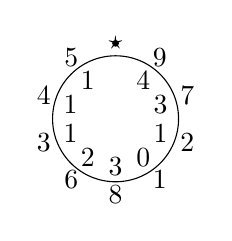
\begin{tikzpicture}
    \draw[black] circle(0.8cm);
    \node[draw=none,minimum size=2cm,regular polygon,regular polygon
    sides=10] (a) {};

    \draw[fill] (a.side 1) circle (1pt) node{\(\star\)};
    \draw[fill] (a.side 2) circle (0pt) node{\(5\)};
    \draw[fill] (a.side 3) circle (0pt) node{\(4\)};
    \draw[fill] (a.side 4) circle (0pt) node{\(3\)};
    \draw[fill] (a.side 5) circle (0pt) node{\(6\)};
    \draw[fill] (a.side 6) circle (0pt) node{\(8\)};
    \draw[fill] (a.side 7) circle (0pt) node{\(1\)};
    \draw[fill] (a.side 8) circle (0pt) node{\(2\)};
    \draw[fill] (a.side 9) circle (0pt) node{\(7\)};
    \draw[fill] (a.side 10) circle (0pt) node{\(9\)};

    \node[draw=none,minimum size=1.25cm,regular polygon,regular polygon
    sides=10] (b) {};
    \draw[fill] (b.side 2) circle (0pt) node{\(1\)};
    \draw[fill] (b.side 3) circle (0pt) node{\(1\)};
    \draw[fill] (b.side 4) circle (0pt) node{\(1\)};
    \draw[fill] (b.side 5) circle (0pt) node{\(2\)};
    \draw[fill] (b.side 6) circle (0pt) node{\(3\)};
    \draw[fill] (b.side 7) circle (0pt) node{\(0\)};
    \draw[fill] (b.side 8) circle (0pt) node{\(1\)};
    \draw[fill] (b.side 9) circle (0pt) node{\(3\)};
    \draw[fill] (b.side 10) circle (0pt) node{\(4\)};
  \end{tikzpicture}
\]
giving \(\charge(\T) = 16\).
\end{example}
\begin{defn}
  We define the charge of a semistandard Young tableau as
  follows. Given a word (tableau) of partition weight,
  \begin{enumerate}
  \item Extract the ``standard'' (permutation) subwords.
  \item Compute charge on each of these subwords.
  \item Sum up each of the separate charges to get the charge.
  \end{enumerate}
\end{defn}
\begin{example}
  Let \[
    \T = \ytableaushort{5,3444,22333,1111224}
  \]
  Then, we draw the reading word on a charge circle and find the
  standard subwords, labeled in different colors and done
  successively for clarity. \[
    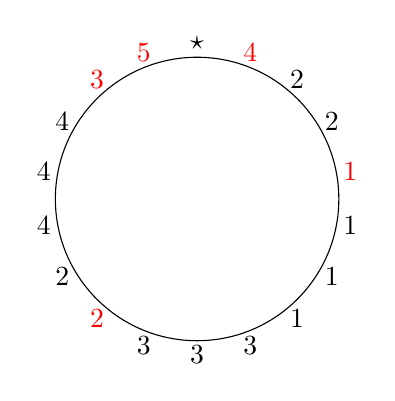
\begin{tikzpicture}
    \draw[black] circle(1.8cm);
    \node[draw=none,minimum size=4cm,regular polygon,regular polygon
    sides=18] (a) {};

    \draw[fill] (a.side 1) circle (0pt) node{\(\star\)};
    \draw[fill] (a.side 2) circle (0pt) node[red]{\(5\)};
    \draw[fill] (a.side 3) circle (0pt) node[red]{\(3\)};
    \draw[fill] (a.side 4) circle (0pt) node{\(4\)};
    \draw[fill] (a.side 5) circle (0pt) node{\(4\)};
    \draw[fill] (a.side 6) circle (0pt) node{\(4\)};
    \draw[fill] (a.side 7) circle (0pt) node{\(2\)};
    \draw[fill] (a.side 8) circle (0pt) node[red]{\(2\)};
    \draw[fill] (a.side 9) circle (0pt) node{\(3\)};
    \draw[fill] (a.side 10) circle (0pt) node{\(3\)};
    \draw[fill] (a.side 11) circle (0pt) node{\(3\)};
    \draw[fill] (a.side 12) circle (0pt) node{\(1\)};
    \draw[fill] (a.side 13) circle (0pt) node{\(1\)};
    \draw[fill] (a.side 14) circle (0pt) node{\(1\)};
    \draw[fill] (a.side 15) circle (0pt) node[red]{\(1\)};
    \draw[fill] (a.side 16) circle (0pt) node{\(2\)};
    \draw[fill] (a.side 17) circle (0pt) node{\(2\)};
    \draw[fill] (a.side 18) circle (0pt) node[red]{\(4\)};
  \end{tikzpicture}
  \rightarrow
  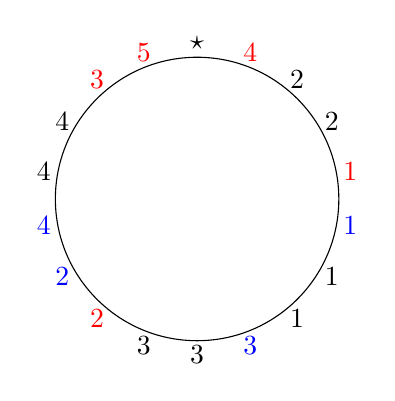
\begin{tikzpicture}
    \draw[black] circle(1.8cm);
    \node[draw=none,minimum size=4cm,regular polygon,regular polygon
    sides=18] (a) {};

    \draw[fill] (a.side 1) circle (0pt) node{\(\star\)};
    \draw[fill] (a.side 2) circle (0pt) node[red]{\(5\)};
    \draw[fill] (a.side 3) circle (0pt) node[red]{\(3\)};
    \draw[fill] (a.side 4) circle (0pt) node{\(4\)};
    \draw[fill] (a.side 5) circle (0pt) node{\(4\)};
    \draw[fill] (a.side 6) circle (0pt) node[blue]{\(4\)};
    \draw[fill] (a.side 7) circle (0pt) node[blue]{\(2\)};
    \draw[fill] (a.side 8) circle (0pt) node[red]{\(2\)};
    \draw[fill] (a.side 9) circle (0pt) node{\(3\)};
    \draw[fill] (a.side 10) circle (0pt) node{\(3\)};
    \draw[fill] (a.side 11) circle (0pt) node[blue]{\(3\)};
    \draw[fill] (a.side 12) circle (0pt) node{\(1\)};
    \draw[fill] (a.side 13) circle (0pt) node{\(1\)};
    \draw[fill] (a.side 14) circle (0pt) node[blue]{\(1\)};
    \draw[fill] (a.side 15) circle (0pt) node[red]{\(1\)};
    \draw[fill] (a.side 16) circle (0pt) node{\(2\)};
    \draw[fill] (a.side 17) circle (0pt) node{\(2\)};
    \draw[fill] (a.side 18) circle (0pt) node[red]{\(4\)};
  \end{tikzpicture}
  \rightarrow
  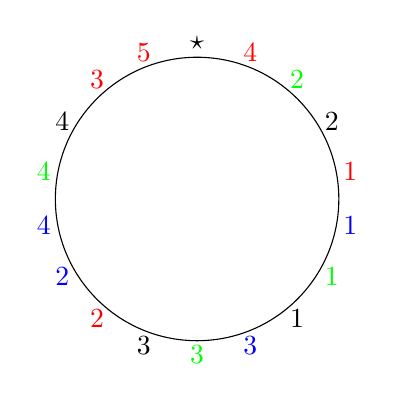
\begin{tikzpicture}
    \draw[black] circle(1.8cm);
    \node[draw=none,minimum size=4cm,regular polygon,regular polygon
    sides=18] (a) {};

    \draw[fill] (a.side 1) circle (0pt) node{\(\star\)};
    \draw[fill] (a.side 2) circle (0pt) node[red]{\(5\)};
    \draw[fill] (a.side 3) circle (0pt) node[red]{\(3\)};
    \draw[fill] (a.side 4) circle (0pt) node{\(4\)};
    \draw[fill] (a.side 5) circle (0pt) node[green]{\(4\)};
    \draw[fill] (a.side 6) circle (0pt) node[blue]{\(4\)};
    \draw[fill] (a.side 7) circle (0pt) node[blue]{\(2\)};
    \draw[fill] (a.side 8) circle (0pt) node[red]{\(2\)};
    \draw[fill] (a.side 9) circle (0pt) node{\(3\)};
    \draw[fill] (a.side 10) circle (0pt) node[green]{\(3\)};
    \draw[fill] (a.side 11) circle (0pt) node[blue]{\(3\)};
    \draw[fill] (a.side 12) circle (0pt) node{\(1\)};
    \draw[fill] (a.side 13) circle (0pt) node[green]{\(1\)};
    \draw[fill] (a.side 14) circle (0pt) node[blue]{\(1\)};
    \draw[fill] (a.side 15) circle (0pt) node[red]{\(1\)};
    \draw[fill] (a.side 16) circle (0pt) node{\(2\)};
    \draw[fill] (a.side 17) circle (0pt) node[green]{\(2\)};
    \draw[fill] (a.side 18) circle (0pt) node[red]{\(4\)};
  \end{tikzpicture}
\]
And thus giving us \[
  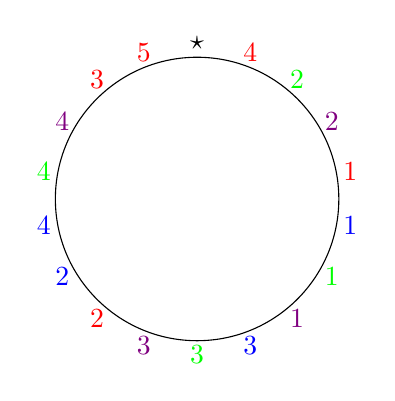
\begin{tikzpicture}
    \draw[black] circle(1.8cm);
    \node[draw=none,minimum size=4cm,regular polygon,regular polygon
    sides=18] (a) {};

    \draw[fill] (a.side 1) circle (0pt) node{\(\star\)};
    \draw[fill] (a.side 2) circle (0pt) node[red]{\(5\)};
    \draw[fill] (a.side 3) circle (0pt) node[red]{\(3\)};
    \draw[fill] (a.side 4) circle (0pt) node[violet]{\(4\)};
    \draw[fill] (a.side 5) circle (0pt) node[green]{\(4\)};
    \draw[fill] (a.side 6) circle (0pt) node[blue]{\(4\)};
    \draw[fill] (a.side 7) circle (0pt) node[blue]{\(2\)};
    \draw[fill] (a.side 8) circle (0pt) node[red]{\(2\)};
    \draw[fill] (a.side 9) circle (0pt) node[violet]{\(3\)};
    \draw[fill] (a.side 10) circle (0pt) node[green]{\(3\)};
    \draw[fill] (a.side 11) circle (0pt) node[blue]{\(3\)};
    \draw[fill] (a.side 12) circle (0pt) node[violet]{\(1\)};
    \draw[fill] (a.side 13) circle (0pt) node[green]{\(1\)};
    \draw[fill] (a.side 14) circle (0pt) node[blue]{\(1\)};
    \draw[fill] (a.side 15) circle (0pt) node[red]{\(1\)};
    \draw[fill] (a.side 16) circle (0pt) node[violet]{\(2\)};
    \draw[fill] (a.side 17) circle (0pt) node[green]{\(2\)};
    \draw[fill] (a.side 18) circle (0pt) node[red]{\(4\)};
  \end{tikzpicture}
  \begin{tikzpicture}
    \draw[fill] (0,0) circle (0pt);
    \draw[fill] (0,2) circle (0pt) node{\(\mapsto\)};
  \end{tikzpicture}
  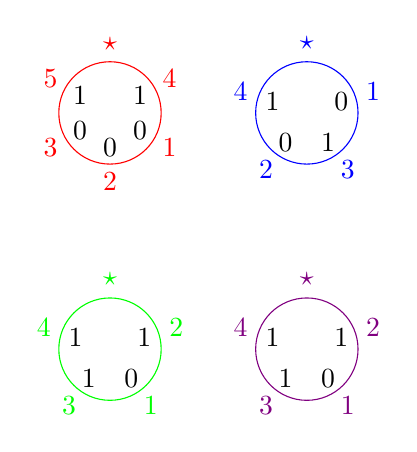
\begin{tikzpicture}
    \draw[red] (0,1.5) circle(0.65cm);
    \node[draw=none, minimum size=2cm, regular polygon, regular
    polygon sides=6] (a) at (0,1.5) {};
    \draw[fill] (a.side 1) circle (0pt) node[red]{\(\star\)};
    \draw[fill] (a.side 2) circle (0pt) node[red]{\(5\)};
    \draw[fill] (a.side 3) circle (0pt) node[red]{\(3\)};
    \draw[fill] (a.side 4) circle (0pt) node[red]{\(2\)};
    \draw[fill] (a.side 5) circle (0pt) node[red]{\(1\)};
    \draw[fill] (a.side 6) circle (0pt) node[red]{\(4\)};

    \node[draw=none, minimum size=1cm, regular polygon, regular
    polygon sides=6] (ain) at (0,1.5) {};
    \draw[fill] (ain.side 2) circle (0pt) node{\(1\)};
    \draw[fill] (ain.side 3) circle (0pt) node{\(0\)};
    \draw[fill] (ain.side 4) circle (0pt) node{\(0\)};
    \draw[fill] (ain.side 5) circle (0pt) node{\(0\)};
    \draw[fill] (ain.side 6) circle (0pt) node{\(1\)};

    
    \draw[blue] (2.5,1.5) circle(0.65cm);
    \node[draw=none, minimum size=1.75cm, regular polygon, regular
    polygon sides=5] (b) at (2.5,1.5) {};
    \draw[fill] (b.corner 1) circle (0pt) node[blue]{\(\star\)};
    \draw[fill] (b.corner 2) circle (0pt) node[blue]{\(4\)};
    \draw[fill] (b.corner 3) circle (0pt) node[blue]{\(2\)};
    \draw[fill] (b.corner 4) circle (0pt) node[blue]{\(3\)};
    \draw[fill] (b.corner 5) circle (0pt) node[blue]{\(1\)};

    \node[draw=none, minimum size=0.9cm, regular polygon, regular
    polygon sides=5] (bin) at (2.5,1.5) {};
    \draw[fill] (bin.corner 2) circle (0pt) node{\(1\)};
    \draw[fill] (bin.corner 3) circle (0pt) node{\(0\)};
    \draw[fill] (bin.corner 4) circle (0pt) node{\(1\)};
    \draw[fill] (bin.corner 5) circle (0pt) node{\(0\)};

    
    \draw[green] (0,-1.5) circle(0.65cm);
    \node[draw=none, minimum size=1.75cm, regular polygon, regular
    polygon sides=5] (c) at (0,-1.5) {};
    \draw[fill] (c.corner 1) circle (0pt) node[green]{\(\star\)};
    \draw[fill] (c.corner 2) circle (0pt) node[green]{\(4\)};
    \draw[fill] (c.corner 3) circle (0pt) node[green]{\(3\)};
    \draw[fill] (c.corner 4) circle (0pt) node[green]{\(1\)};
    \draw[fill] (c.corner 5) circle (0pt) node[green]{\(2\)};

    \node[draw=none, minimum size=0.9cm, regular polygon, regular
    polygon sides=5] (cin) at (0,-1.5) {};
    \draw[fill] (cin.corner 2) circle (0pt) node{\(1\)};
    \draw[fill] (cin.corner 3) circle (0pt) node{\(1\)};
    \draw[fill] (cin.corner 4) circle (0pt) node{\(0\)};
    \draw[fill] (cin.corner 5) circle (0pt) node{\(1\)};

    
    \draw[violet] (2.5,-1.5) circle(0.65cm);
    \node[draw=none, minimum size=1.75cm, regular polygon, regular
    polygon sides=5] (d) at (2.5,-1.5) {};
    \draw[fill] (d.corner 1) circle (0pt) node[violet]{\(\star\)};
    \draw[fill] (d.corner 2) circle (0pt) node[violet]{\(4\)};
    \draw[fill] (d.corner 3) circle (0pt) node[violet]{\(3\)};
    \draw[fill] (d.corner 4) circle (0pt) node[violet]{\(1\)};
    \draw[fill] (d.corner 5) circle (0pt) node[violet]{\(2\)};

    \node[draw=none, minimum size=0.9cm, regular polygon, regular
    polygon sides=5] (din) at (2.5,-1.5) {};
    \draw[fill] (din.corner 2) circle (0pt) node{\(1\)};
    \draw[fill] (din.corner 3) circle (0pt) node{\(1\)};
    \draw[fill] (din.corner 4) circle (0pt) node{\(0\)};
    \draw[fill] (din.corner 5) circle (0pt) node{\(1\)};
  \end{tikzpicture}
\]
Thus, the charge would be \(2+2+3+3=10\). 
\end{example}
\begin{example}
  Our theorem says that
  \begin{align*}
        s_{21} & = \sum_{\text{partition }\mu}\left(\sum_{\T \in \SSYT((2,1), \mu)}
                 t^{\charge(\T)}\right) P_\mu(x;t)\\
    & = \left( \sum_{\T \in
        \SSYT((2,1),(2,1))} t^{\charge(\T)}\right) P_{21}(x;t) +
    \left( \sum_{\T \in \SSYT((2,1),(1,1,1))} t^{\charge(\T)} \right) P_{111}(x;t)
  \end{align*}
  Thus, we can now use our theorem to compute \[
    s_{21} = t^0 P_{21}(x;t) + (t^2+t)P_{111}(x;t)
  \]
  since \[
    \begin{cases}
      \ytableaushort{2,11} \text{ has charge }0\\
      \\
      \ytableaushort{3,12} \text{ has charge }1\\
      \\
      \ytableaushort{2,13} \text{ has charge }2
    \end{cases}
  \]
\end{example}
\begin{rmk}
  It should be noted that all Hall-Littlewood polynomials are actually
  special cases of LLT polynomials. \todo{However, I do not know how
    to prove this.}
\end{rmk}
\begin{bibdiv}
  \begin{biblist}
    \bib{fulton}{book}{
      author={Fulton, William}
      title={Young Tableaux}
      year={1997}
    }
    \bib{haglund}{book}{
      author={Haglund, J.}
      title={The \(q,t\)-Catalan Numbers and the Space of Diagonal
        Harmonics}
      year={2008}
    }
    \bib{haglund-et-al}{article}{
      author={Haglund, J.}
      author={Haiman, M.}
      author={Loehr, N.}
      author={Remmel, J.B.}
      author={Ulyanov, A.}
      title={A combinatorial formula for the character of the diagonal
        coinvariants}
      year={2004}
    }
    \bib{macdonald}{book}{
      author={Macdonald, I.G.}
      title={Symmetric Functions and Hall Polynomials}
      year={1979}
      note={2nd Edition, 1995}
    }
    \bib{stembridge}{article}{
      author={Stembridge, John R.}
      title={A Concise Proof of the Littlewood-Richardson Rule}
      year={2002}
      journal={The Electronic Journal of Combinatorics}
    }
  \end{biblist}
\end{bibdiv}

\end{document}